\documentclass{report}
\usepackage{amsfonts,amsthm,amsmath,latexsym,amssymb}
\usepackage[margin=1.5in]{geometry}
\usepackage{complexity}
\usepackage{graphicx}
\usepackage[titles,subfigure]{tocloft}
\usepackage{scribe-book}
\usepackage[lined,boxed]{algorithm2e}


\usepackage{caption}
\usepackage{subcaption}
\usepackage{float}

\newcommand{\CYCLE}{{\sf CYCLE~}}
\newcommand{\FPSPACE}{{\sf FPSPACE~}}
\newcommand{\N}{{\mathbb{N}}}
\newcommand{\Z}{{\mathbb{Z}}}
\newcommand{\F}{{\mathbb{F}}}

%% For xy matrix
\input xy
\xyoption{all}
\CompileMatrices

\usepackage{tikz}
\usetikzlibrary{arrows}

\usetikzlibrary{calc,through,backgrounds,decorations.pathmorphing}

% Shows lecture titles and sections. Set 0 to list only chapters.
\setcounter{tocdepth}{1}

\begin{document}
\newpage
\setcounter{page}{1}
\pagenumbering{roman}  % Roman numbering in intro portion.
\include{front-page}

\newpage
\listofscribe          % For automatic scribe list generation.

\newpage
\tableofcontents

\setcounter{page}{1}
\pagenumbering{arabic}  % Arabic page numbering for lectures.

% Autogenerated using Makefile. DO NOT EDIT
\newpage \include{Lecture04-Dinesh/lecture04}
\newpage \include{Lecture05-Prasun/lecture05}
\newpage \include{Lecture06-Sunil/lecture06}
\newpage \include{Lecture07-Dinesh/lecture07}
\newpage 
\newcommand{\sP}{\#\P} %% The class #P as it is not defined in complexity.sty
\Lecture{Akshay Degwekar, Devanathan.T}{Jan 17, 2012}{8}{Permanent Computation is \sP-Complete}

\newcommand{\per}{{\sf Per}} % Permanent is defined as an operator.
\newcommand{\wt}{{\sf Weight}} % Weight is defined as an operator.
\newcommand{\integer}{\mathbb{Z}}

In this lecture, we define the permanent of a matrix and study the complexity of computing the permanent for various classes of matrices. Finally we prove a theorem by Valiant that $\per(A)$ is \sP-Complete.

\section{Definitions}
\begin{definition}
\textbf{Permanent } Given a matrix $A_{n \times n}$, Let $S_n$ be the set of
all permutations of $\{1,2,\ldots,n\} = [n]$. Then
\begin{equation}
\per(A) = \sum_{\sigma \in S_n } \prod_{i=1}^n A_{i,\sigma(i)} 
\end{equation}
\end{definition}

Earlier, we have seen a characterization of the permanent as the number of perfect matchings in a graph G. To prove the result, we characterize the permanent using \textbf{Cycle Covers}.

\begin{definition}
\textbf{Cycle Cover } A Cycle Cover $C$ of a directed graph G is a set of pairwise disjoint simple cycles such that each vertex lies in exactly one cycle in $C$.

Note that we allow self-loops as simple cycles.

\xymatrix{
		  & 3 \ar[dr]&	            &   	&	7\ar[dr] \\
2 \ar[ur]& 		 &4\ar[dl]\ar[r]&6\ar[ur]  && 8\ar[dl] \\
&1 \ar[ul]&&&5\ar[ul]&\\}
Has a cycle cover $\big{\{}\{1,2,3,4\},\{5,6,7,8\}\big{\}}$.

\begin{definition}
\textbf{Weight of a Cycle Cover} Given a Graph $G(V,E)$, let $C={C_1, C_2, \dots C_l}$ be any cycle cover
\begin{equation}
\textbf{Weight of Cycle - } \wt(C_i) = \prod_{e\in E}w(e)
\end{equation}
\begin{equation}
\textbf{Weight of Cycle Cover - } \wt(C_i) = \prod_{c\in C}\wt(c)
\end{equation}
\end{definition}


%%That is, In a graph $G(V,E)$, $C = {C_1, C_2, \dots C_l}$ is a cycle cover iff $\forall i,j \quad C_i\cap C_j = \phi$ and $v\in V, \, \exists ! j $ such that $•$ $C_j$ is a 

\end{definition}

\begin{lemma}
Let $G(V,E)$ be a graph with adjacency matrix $A$. 
$A \in \mathbb{Z}^{n\times n}$. Then 
\begin{equation}
	\per(A) = \sum_{\substack{C \text{ is a} \\ \text{Cycle Cover}}} \wt(C)
\end{equation}
\end{lemma}
\begin{proof}
Consider a single term from the permanent - $\sum^n_{i=1}A_{i,\sigma(i)}$.

We can view $\sigma$ as a cycle cover as follows. 

First we decompose $\sigma$ into cycles of the form $a, \sigma(a),
\sigma^2(a)\dots \sigma^k(a) = a$. Now each cycle in the permutation can be
viewed as a cycle in the graph G, the edges being 
\[ \big{\{} (1, \sigma(1)),(2, \sigma(2)), \dots (n, \sigma(n)) \big{\}} \]
This is the required cycle cover. 

For the other direction, some of the cycle covers generated from permutation
might not be valid as some edges are absent. In that case, we just see that 
their weight is 0 as $A_{i,j} = 0$ for the missing edge $(i,j)$. And in the 
case that it is a valid cover, $\wt(C) = \prod_{i\in[n]}A_{i,\sigma(i)}$, because both of them are exactly the product of the corresponding edges.

This shows a bijective correspondence between the permutations and the cycle
covers which completes the proof.
\end{proof}

%%%%%%%%%%%%%%%%Some explanation and notes are required here.

\begin{exercise}
Let $\mathbb{Z}_+$ denote the non negative integers.
Using the previous construction involving cycle covers, 
show that for $A\in \mathbb{Z}_{+}^{n\times n}, \per(A)\in \FP^{\sP}$.

% This problem is also a part of the first problem set.
\end{exercise}


\begin{exercise}
Is the reduction from $\SAT$ to $3\SAT$ parsimonious? If yes, show that
$\#3\SAT$ is $\sP$-complete. 
\end{exercise}

\section{Proof of harndess of Permanent computation}
%Now, we move towards the final part of the lecture - the result by Valiant, that $Per$ is $\sP-Hard$. The proof given here is due to Del.... %add the citations here for both the papers.
In this section, we show that computing permanant of a $0-1$ matrix is $\sP$
complete. The result is due to Valiant~\cite{valiant79}. The proof presented
here is from Dell. et.al~\cite{dell12}. 

We will show this by using a gadget construction.

\begin{theorem}
$\#3\SAT\in \FP^{\per}$
\end{theorem}
\begin{proof}
Consider a formula $\phi $ in $3\SAT$. $\phi = C_1\wedge C_2 \dots C_m$ where $C_i = l_{i,1}\vee l_{i,2} \vee l_{i,3}$.

We will construct a directed graph $G$ such that $A_G$ is the adjacency matrix of $G$, such that $A_G \in \{-1,0,1\}^{n\times n}$ and also, $\per(A_G)=(-2)^k(\#\phi)$ where $(\#\phi)$ is the number of satisfying assignments of $\phi$ and $k$ is a quantity that we specify later.

\begin{lemma}
Let $\#x$ be the number of times a variable $x$ occurs in $\phi$. 

Then $\phi$ can be converted to $\phi'$ such that $\forall x$, $k = \#x=\# \overline{x}$ and $\#phi = \# phi'$
\end{lemma}

\begin{proof}
 We first observe that if $\# x \not = \# \overline{x}$. Then this imbalance can be removed by adding terms of the form $(x\vee x\vee \overline{x})$ and/or $(x\vee \overline{x}\vee \overline{x})$ because they add or decrease the relative number of $x$ compared to $\overline{x}$.
 
 Now, we assume that $\forall x, \#x = \# \overline{x}$.
 Now to compensate for relative differences between $x, y$ we add terms of the form $(x\vee \overline{x}\vee \overline{y})\wedge (x\vee \overline{x}\vee \overline{y})$ to increase the number of $x$ and the other way to decrease.
 
 And we just note that the number of solutions is invariant because each of the added terms are always true.
 
 This completes the lemma.
 \end{proof}
  
  We will be constructing the graph from three gadgets - Variable Gadget, Clause Gadget and the Equality Gadget.

%%% The gadgets  
\begin{figure}[h!]
\centering
%%%%%%%Variable Gadget
\begin{subfigure}[b]{0.3\textwidth}
\xymatrix{ 
	{\bullet}  \ar @/_/ [dd]_x  \ar @/^/ [dd]^{\overline{x}} \\ \\
	{\bullet} \ar [uu]}
	\caption{Variable Gadget}
\end{subfigure} 
%%%%%%%Clause Gadget
\begin{subfigure}[b]{0.3\textwidth}
\centering
 \xymatrix{ 
	 & {\bullet}  \ar @/^/ [d]   \ar @/_/ [ddl]_{\overline{l_1}} & \\ 
	 & {\bullet}  \ar @/^/ [u]  \ar @/^/ [dl]  \ar @/^/ [dr] & \\
{\bullet}\ar @/_/ [rr]_{\overline{l_3}} \ar @/^/ [ur] & & {\bullet}  \ar @/^/ [lu] \ar @/_/ [uul]_{\overline{l_2}} \\	
	}
	\caption{Clause Gadget}
\end{subfigure}
%%%%%%%Equality Gadget
\begin{subfigure}[b]{0.3\textwidth}
\centering
 \xymatrix{ 
	\ar @/_/[ddr] & & {\bullet} \ar@(ul,ur)^{-1} \ar @/_/[ddr] \ar @/_/ [ddl]& & \ar @/^/[ddl] \\ 
	\\
	\ar @/^/[r] & {\bullet}  \ar@(dl,dr)_{1}\ar @/_/ [uur]  \ar @/_/ [rr] & &  {\bullet}  \ar @/_/[uul]  \ar @/_/[ll] \ar@(dl,dr)_{1} & \ar @/_/[l] }
	
	\caption{Equality Gadget}
\end{subfigure}
\caption{The Gadgets}
\label{fig1Gadgets}
\end{figure}

Now, we consider the construction of the graph.

For each variable pair $(x, \overline{x})$ we have one variable gadget. Each clause has a Clause Gadget and the equality gadget is used to join each variable with all the clauses the variable is in.

The equality gadget is represented as a black box as follows -
\begin{figure}[h!]
\centering
\begin{subfigure}[b]{0.3\textwidth}
\centering
 \xymatrix{ 
	\ar @/_/[ddr] & & {\bullet} \ar@(ul,ur)^{-1} \ar @/_/[ddr] \ar @/_/ [ddl]& & \ar @/^/[ddl] \\ 
	\\
	\ar @/^/[r] & {\bullet}  \ar@(dl,dr)_{1}\ar @/_/ [uur]  \ar @/_/ [rr] & &  {\bullet}  \ar @/_/[uul]  \ar @/_/[ll] \ar@(dl,dr)_{1} & \ar @/_/[l] }
	
	\caption{Equality Gadget}
\end{subfigure}
\begin{subfigure}[b]{0.3\textwidth}
\centering
\xymatrix{ 
	\ar @/_/[drr] & \ar @{-} [rrr] \ar @{-} [dd]& & &\ar @{-} [dd] & \ar @/^/[dll]\\
 & & \ar @/_/[dll]&\ar @/^/[drr] & & \\
 & \ar @{-} [rrr]& & & &\\
}	
	\caption{Equality Gadget Representation}
\end{subfigure}
\caption{Equality Gadget Blackbox representation}
\label{fig:EqBlackbox}
\end{figure}

The way we connect a variable and a clause is shown in the next figure. Here $\overline{x}$ is the literal $l_1$ in the clause. 

\begin{figure}[h!]
\centering

\begin{subfigure}[b]{0.3\textwidth}
\centering
\xymatrix{ 
{a}  \ar @/_/ [dd]_x  \ar @/_/[drr]^{u} & \ar @{-} [rrr] \ar @{-} [dd]& & &\ar @{-} [dd] &  & 
{\bullet} \ar @/^/[dlll]^{u'}  \ar @/^/ [d] &  \\ 
 & & \ar @/_/[dll]^{v} &\ar @/^/[drr]^{v'} & &  &  
{\bullet}  \ar @/^/ [u]  \ar @/^/ [dl]  \ar @/^/ [dr] & \\
{b} \ar [uu] & \ar @{-} [rrr]& & & &
{\bullet} \ar @/_/ [rr]^{\overline{l_3}} \ar @/^/ [ur] & & {\bullet} \ar @/_/ [uul]^{\overline{l_2}}  \ar @/^/ [lu] \\	
}	
\end{subfigure}
\caption{Connection between variables and clauses.}
\label{VarClauseConnection}
\end{figure}

When the same variable appears in multiple clauses, we split the edge representing the variable and attach multiple equality gadgets. The next figure shows the split.

\begin{figure}[ht!]
\begin{subfigure}[b]{0.3\textwidth}
\xymatrix{ 
	{\bullet}  \ar @/_/ [ddd]_{\overline{x}}  \ar @/_/ [dr] & & & &  \\ 
& Equality Gadget \ar @/_/ [d] \ar @/_/ [rr] & & Clause Gadget \ar @/_/ [ll]& &\\
& Equality Gadget  \ar @/_/ [dl] \ar @/_/ [rr] & & Clause Gadget \ar @/_/ [ll]& & \\
	{\bullet} \ar [uuu]}
	\label{fig:subfigure1}
\end{subfigure}
	\caption{One variable occurring in multiple clauses.}
\end{figure}

This essentially completes the construction. We will prove the correctness of the construction in a series of claims.
\begin{claim}
Any cycle cover can either use the edge $x$ or $\overline{x}$ in the variable gadget, but not both.
\end{claim}
\begin{proof}
If a cycle cover used both the edges, then the vertices would be covered twice. 
\end{proof}

\begin{claim}
Each assignment corresponds to atleast one cycle cover. 
\end{claim}
\begin{proof}
For each variable, choose $x$ or $\overline{x}$ based on the assignment. And for each clause choose the cycle $l_1 \rightarrow l_2 \rightarrow l_3$ and choose self-loops everywhere else.
\end{proof}

We will derive a much precise correspondence in the remaining proof.


\begin{claim}
In any cycle cover C, either both $u,v$ are used, or neither $u,v$ are used.
\end{claim}
\begin{proof}
The proof is just a verification, We see in \ref{VarClauseConnection} that if the edge $u$ is used, edge $(b,a)$ will have to be used, and to complete a cycle, we will need $v$ to complete the cycle as the edge $x$ cannot be used. 

The proof holds unmodified for edges $u',v'$ too.
\end{proof}

\begin{claim}
If both $u,v$ and $u',v'$ edges are used in the cycle cover, then the $-1$ valued self-loop has to be chosen in the cycle cover. 
\end{claim}

\begin{claim}
If edges $u,v$ are used while $u',v'$ are not used, the corresponding Cycle Covers contribute weight 0.
\end{claim}
\begin{proof}
We just observe that there are two components one contributing $+1$ and the other as $-1$ in the cycle weight. Cycle covers are marked in double lines.

\begin{figure}[H]
\begin{subfigure}[b]{0.3\textwidth}
\centering
 \xymatrix{ 
	\ar @{=>} @/_/[ddr]^{u}  & & {\bullet} \ar@(ul,ur)^{-1} \ar @{=>}@/_/[ddr] \ar   @/_/ [ddl]& & \ar @/^/[ddl]_{u'} \\ 
	\\
	\ar @{<=} @/^/[r]_{v} & {\bullet}  \ar@(dl,dr)_{1}\ar  @/_/ [uur]  \ar @/_/ [rr] & &  {\bullet}  \ar @{=>} @/_/[uul]  \ar @/_/[ll] \ar@(dl,dr)_{1} & \ar @/_/[l]^{v'} }
	\caption{Weight +1}
\end{subfigure}
\begin{subfigure}[b]{0.3\textwidth}
\centering
 \xymatrix{ 
	\ar @{=>}@/_/[ddr]^{u}  & & {\bullet} \ar@{=>}@(ul,ur)^{-1} \ar @/_/[ddr] \ar @/_/ [ddl]& & \ar @/^/[ddl]_{u'} \\ 
	\\
	\ar @{<=}@/^/[r]_{v} & {\bullet}  \ar@(dl,dr)_{1}\ar @/_/ [uur]  \ar @/_/ [rr] & &  {\bullet}  \ar @/_/[uul]  \ar @/_/[ll] \ar@{=>}@(dl,dr)_{1} & \ar @/_/[l]^{v'} }
	\caption{Weight -1}
\end{subfigure}
\caption{Only one of the two sets of edges are present}
\end{figure}
\end{proof}


\begin{claim}
If both $u,v$ and $u',v'$ are not used, then the Cycle Covers have a contribution of 2 from this gadget. 
\end{claim} 
\begin{proof}
The figure \ref{Fig6} contains all the possible cycle covers of the gadget. Their contributions sum upto 2.
\begin{figure}[h]
\begin{subfigure}[b]{0.3\textwidth}
\centering
 \xymatrix{ 
	\ar  @/_/[ddr]^{u}  & & {\bullet} \ar @{=>}@(ul,ur)^{-1} \ar @/_/[ddr] \ar   @/_/ [ddl]& & \ar @/^/[ddl]_{u'} \\ 
	\\
	\ar  @/^/[r]_{v} & {\bullet}  \ar @{=>}@(dl,dr)_{1}\ar  @/_/ [uur]  \ar @/_/ [rr] & &  {\bullet}  \ar @/_/[uul]  \ar @/_/[ll] \ar @{=>}@(dl,dr)_{1} & \ar @/_/[l]^{v'} }
	\caption{Weight -1}
\end{subfigure}
\begin{subfigure}[b]{0.3\textwidth}
\centering
 \xymatrix{ 
	\ar @/_/[ddr]^{u}  & & {\bullet} \ar@{=>}@(ul,ur)^{-1} \ar @/_/[ddr] \ar @/_/ [ddl]& & \ar @/^/[ddl]_{u'} \\ 
	\\
	\ar @/^/[r]_{v} & {\bullet}  \ar@(dl,dr)_{1}\ar @/_/ [uur]  \ar@{=>}@/_/[rr] & &  {\bullet}  \ar @/_/[uul]  \ar@{=>}@/_/[ll] \ar@(dl,dr)_{1} & \ar @/_/[l]^{v'} }
	\caption{Weight -1}
	\end{subfigure}
\begin{subfigure}[b]{0.3\textwidth}
\centering
 \xymatrix{ 
	\ar  @/_/[ddr]^{u}  & & {\bullet} \ar @(ul,ur)^{-1} \ar @{=>}@/_/[ddr] \ar   @/_/ [ddl]& & \ar @/^/[ddl]_{u'} \\ 
	\\
	\ar  @/^/[r]_{v} & {\bullet}  \ar @{=>}@(dl,dr)_{1}\ar  @/_/ [uur]  \ar @/_/ [rr] & &  {\bullet}  \ar @{=>}@/_/[uul]  \ar @/_/[ll] \ar @(dl,dr)_{1} & \ar @/_/[l]^{v'} }
	\caption{Weight 1}
\end{subfigure}	
\begin{subfigure}[b]{0.3\textwidth}
\centering
 \xymatrix{ 
	\ar  @/_/[ddr]^{u}  & & {\bullet} \ar @(ul,ur)^{-1} \ar @/_/[ddr] \ar@{=>}@/_/ [ddl]& & \ar @/^/[ddl]_{u'} \\ 
	\\
	\ar  @/^/[r]_{v} & {\bullet}  \ar@(dl,dr)_{1}\ar  @{=>}@/_/ [uur]  \ar @/_/ [rr] & &  {\bullet}  \ar @/_/[uul]  \ar @/_/[ll] \ar @{=>}@(dl,dr)_{1} & \ar @/_/[l]^{v'} }
	\caption{Weight 1}
\end{subfigure}	
\begin{subfigure}[b]{0.3\textwidth}
\centering
 \xymatrix{ 
	\ar  @/_/[ddr]^{u}  & & {\bullet} \ar @(ul,ur)^{-1} \ar @/_/[ddr] \ar@{=>}@/_/ [ddl]& & \ar @/^/[ddl]_{u'} \\ 
	\\
	\ar  @/^/[r]_{v} & {\bullet}\ar@(dl,dr)_{1}\ar@/_/ [uur]\ar@{=>}@/_/ [rr] & &  {\bullet}  \ar@{=>}@/_/[uul]  \ar @/_/[ll] \ar @(dl,dr)_{1} & \ar @/_/[l]^{v'} }
	\caption{Weight 1}
\end{subfigure}	
\begin{subfigure}[b]{0.3\textwidth}
\centering
 \xymatrix{ 
	\ar@/_/[ddr]^{u}  & & {\bullet} \ar@(ul,ur)^{-1} \ar@{=>}@/_/[ddr] \ar@/_/ [ddl]& & \ar @/^/[ddl]_{u'} \\ 
	\\
	\ar  @/^/[r]_{v} & {\bullet}\ar@(dl,dr)_{1} \ar@{=>}@/_/[uur] \ar@/_/[rr] & &  {\bullet}\ar@/_/[uul]  \ar@{=>}@/_/[ll] \ar@(dl,dr)_{1} & \ar@/_/[l]^{v'} }
	\caption{Weight 1}
\end{subfigure}	
\caption{The weights sum upto 2}
\label{Fig6}
\end{figure}
\end{proof}

\begin{claim}
	Weight of each cycle cover is $(-2)^{kn}$
\end{claim}
\begin{proof}
We want to claim that if a variable $x$ is assigned value $1$, then all the equality gadgets for $x$ will contribute $1$ to the weight because $u,v$ and $u',v'$ will both be a part of the cycle cover for each of the gadgets, if just one pair is in the cycle cover, we have seen that those covers would contribute 0 to the weight. 

Also, the gadgets that correspond to $\overline{x}$ will not have either $u,v$ or $u',v'$ being used - because, $u,v$ cannot be used as $x$ edge will be used, hence $\overline{x}$ cannot be used. Now, if $u',v'$ are used, those cycles will have 0 weight as seen in the observation.

So, the only possibility there is both $u,v$ and $u',v'$ are not used. In that case, the contribution would be $2$ for each gadget. As there are $k$ such gadgets, we will have a contribution of $2^k$ from these. 

So, multiplying them would give us, that each variable pair $x,\overline{x}$ contribute exactly $(-2)^k$ to the weight. Hence the cycle cover would have a weight of exactly $(-2)^{kn}$.

So, We sum them up over all the possible assignments to get the required result. This completes the proof.

\end{proof}

So, we have the result -
\begin{equation}
{\sum_{\text{C is a Cycle Cover}} \wt(C) }= \per_{-1,0,1}(A)
\end{equation}

Hence computing $\#\SAT$ reduces to computing $\per_{-1,0,1}$. This completes the proof. 
\end{proof}

Now we will first show that $\per_{-1,0,1}$ reduces to $\per_{0,1,\dots n}$ and finally show that $\per_{0,1,\dots n}$ reduces to $\per_{0,1}$ and hence completing the theorem.

\begin{theorem}
$\per_{-1,0,1} \in \FP^{\per_{0,1,\dots n}}$.
\end{theorem}
\begin{proof}
 The first thing we observe is that all the -1 terms in the adjacency matrix $A$ represent self-loops because in the construction, $-1$ was the edge weight of only one self-loop.
 
 Consider $\per(A)$ as a polynomial in $x$ where each $-1$ is replaced by $x$ denoted by $p(x)$ 
 
 Now we just observe that, using ${\per_{0,1,\dots n}}$ as an oracle, we can find $p(0), p(1), ... p(n)$. Also, degree of p $\leq n$ because x occurs only in the diagonal entries, hence only n $x $ can be present. 
 
 So, now we just use Lagrange Interpolation to find the polynomial $p$. This can be done in poly time. Once this is done, $\per_{-1,0,1}(A) = p(-1)$, which can be computed easily.
 
 This completes the reduction.
\end{proof}

In the final reduction, we show that $\per_{0,1,\dots n} \in \FP^{\per_{0,1}}$, and that $\per_{0,1}$ is as hard as the other $\per$ computations. 

\begin{theorem}
$\per_{0,1,\dots n} \in \FP^{\per_{0,1}}$
\end{theorem}
\begin{proof}
This proof involves substituting the $-1$ self-loop with a gadget so that we can compute the values of the polynomial $p(x)$ at points $x=0, x=1, \dots x=n$.

The gadget we use is - 
Consider any $a = (a_k, a_{k-1}\dots a_{0})_2$ in base $2$ where $a\in \{0, 1, \dots n\}$. Now we want to replace the self-loop of weight $a$ with the gadget, so that the gadget contributes exactly $k$ weight to the Cycle cover. 

\begin{figure}[ht!]
\xymatrix{
\ar[r]^{1} & \ar@/^/[d]^{a_0} \ar@/_/[r]^{1} \ar@/^/[r]^{1} & \ar@(ul,ur) \ar@/^/[dl]^{a_1} \ar@/_/[r]^{1} \ar@/^/[r]^{1}  & \ar@(ul,ur) \ar@/^/[dll]^{a_2} \ar@[--][r] & \ar@(ul,ur) \ar@/^/[dlll]^{a_{k-1}}   \ar@/_/[r]^{1} \ar@/^/[r]^{1} & \ar@(ul,ur) \ar@/^/[dllll]^{a_{k}} \\ 
& \ar[ul]^{1} & & \\
}
\end{figure}

The gadget has precisely $n$ cycles of weight $1$ each. This gadget can be used to replace the self loop and then query the $\per_{0,1}$ oracle. 

This completes the reduction. Hence proved.
\end{proof}


\newpage \include{Lecture09-Balagopal/lecture09}
\newpage \Lecture{Sunil K S}{Jan 24, 2012}{10}{Polynomial Identity Testing}

Towards the end of last lecture, we introduced the following problem :
{\em Given a polynomial $p$, test if it is identically zero}. That is,
do all the terms cancel out and become the zero polynomial. Described
as a language :
$$\textrm{\sc PIT}=\{ p ~|~p \equiv 0\}$$
We also saw some easy cases of the problem:
\begin{enumerate}
\item When it is given as a sum of monomials: Given $p$, run over the
  input to figure out the coefficient of each monomial, and if all of
  them turn out to be zero, then report that $p$ is in {\sc PIT}. This
  algorithm runs in $O(n^2)$ time.
\item When it is given as a Black Box: In uni-variate case, check
  $p(x)$ for $d+1$ different points where $d$ is the degree bound. If
  the polynomial is not equivalent to zero, then at-least one of the
  steps gives a non-zero value. Indeed, if the polynomial is zero,
  then all the $(d+1)$ evaluations will result in a zero value. Thus
  the algorithm is correct and runs in time $O(d)$ where $d$ is the
  degree of the polynomial.
\end{enumerate}

As we observed, this strategy could not be generalized in
multi-variate case. We took an example as $p(x_1,x_2) = x_1x_2$. For
the assignment $x_1=0$, whatever $x_2$ chose, the value will always be
0. However, if $p \equiv 0$, no matter what we choose as the
substitution for $x_1$, and $x_2$, the polynomial will be identically
zero.

The strategy that we will follow is as follows: If the total degree of
the polynomial is $\leq d$, and if $S \subseteq \F$, such that
$|S|\geq 2d$, instead of picking elements arbitrarily, we pick
elements uniformly at random from $S$. Indeed, there may be many
choices for the values which may lead to zero. But how many?
%Here by increasing the size of $S$, we can improve the probability.
% IMPRECISE statement.

\begin{lemma}[Schwartz-Zippel Lemma]
Let $p(x_1, x_2, \cdots , x_n)$ be a non-zero polynomial over a field
$\mathbb{F}$. Let $S\subseteq \mathbb{F}$
$$Pr[p(\bar{a}=0]\leq \frac{d}{|S|}$$
\end{lemma}
%It also shows that the number of solutions for $P(\bar{a})$ if $\leq d|S|^{(n-1)}$.
\begin{proof}
(By induction on $n$) For $n=1$: For a univariate polynomial $p$ of
  degree $d$, there are $\leq d$ roots. Now in the worst case the set
  $S$ that we picked has all $d$ roots. Thus for a random choice of
  substitution for the variable from $S$, the probability that it is a zero of
  the polynomial $p$ is at most $\frac{d}{|S|}$.

For $n>1$, write the polynomial $p$ as a univariate polynomial in $x_1$ with coefficients as polynomials in the variables $p(x_2, \ldots, x_n)$.
$$ \displaystyle \sum_{j=0}^{d}x_1^jp_j(x_2, x_3, \ldots, x_n)$$

For example: $x_1x_2^2+x_1^2x_2x_3+x_3^2=(x_2x_3)x_1^2+(x_2^2)x_1+x_1^0(x_3^2)$.

To analyse the probability that we will choose a zero of the
polynomial (even though the polynomial is not identically zero). For a
choice of the variables as $(a_1, a_2, \cdots, a_n)\in S^n$, we ask
the question : how can $p(a_1, a_2, \cdots, a_n)$ be zero? It could be
because of two reasons:

\begin{enumerate}
\item $\forall j~:~1 \le j \le n , ~~ p_j(a_2, a_3, \ldots , a_n)=0$.
% In this case whatever $(a_2, a_3, \cdots , a_n)=0$, polynomial will be zero.
\item %$(a_2, a_3, \cdots , a_n)=0$.
Some coefficients $p_j(a_2, a_3, \ldots , a_n)=0$ are non-zero, but
the resulting univariate polynomial in $x_1$ evaluates to zero upon
substituting $x_1 = a_1$.
\end{enumerate}

Now we are ready to calculate $Pr [ p(a_1, a_2, \ldots, a_n) = 0 ]$.
%\begin{eqnarray*}
For a random choice of $(a_1, \ldots, a_n)$.
Let $A$ denote the event that the polynomial $p(a_1, \ldots, a_n) = 0$.
Let $B$ denote the event that $\forall j~:~1 \le j \le n ,~~p_j(a_2, a_3, \cdots , a_n)=0$.
Now we simply write : $Pr[A] = Pr[A \land B]+Pr[A\land \bar{B}]$.

We calculate both the terms separately: $Pr[A \land B] = Pr[B].Pr[A|B]
= Pr[B]$ where the last equality is because $B \implies A$.  Let
$\ell$ be the highest power of $x_1$ in $p(x)$. That is $p_\ell \ne
0$. Since the event $B$ insists that for all $j$, $p_j(a_2, a_3,
\ldots , a_n)=0$, we have that $Pr[B] \leq Pr[p_\ell(a_1, a_2, \ldots,
  a_n) \ne 0]$.  By induction hypothesis, since this polynomial has
only $n-1$ variables and has degree at most $\frac{d -
  \ell}{S}$. Thus, $Pr[B] \le \frac{d - \ell}{S}$.

To calculate the other term,
\begin{eqnarray*}
Pr[A \cap \bar{B}] & = & Pr[\bar{B}].Pr[A|\bar{B}] \le Pr[A|\bar{B}] \le \frac{\ell}{|S|}
\end{eqnarray*}
where the last inequality holds because the degree of the non-zero
univariate polynomial after substituting for $a_2, \ldots, a_n$ is at
most $\ell$ and hence the base case applies.
\end{proof}

This suggests the following efficient algorithm for solving PIT. Given $d$ and a
blackbox evaluating the polynomial $p$ of degree at most $d$.

\begin{figure}[ht]
{\tt \obeyspaces \obeylines
1. Choose $S \subseteq \mathbb{F}$ of size $\ge 4d$.
1. Choose $(a_1, a_2, \ldots, a_n) \in_R S^n$.
2. Evaluate $p(a_1, a_2, \ldots a_n)$ by querying the blackbox.
3. If it evaluates to 0 accept else reject.
}
\caption{A randomized algorithm for multivariate polynomial identity testing}
\end{figure}

The algorithm is clearly running in polynomial time. The following
Lemma states the error probability and follows from the
Schwartz-Zippel Lemma that we saw before.
\begin{lemma}
There is a randomized polynomial time algorithm $A$, which, given a black
box access to a polynomial $p$ of degree $d$ ($d$ is also given in unary), answers whether the polynomial is identically zero or not,
with probability at least $\frac{3}{4}$.
%\[ p \not\equiv 0 \implies \textrm{ Pr[$A$ accepts] $\ge \frac{3}{4}$} \]
%\[ p \equiv 0 \implies \textrm{ Pr[$A$ accepts] $= 0$.} \]
\end{lemma}

Notice that in fact the lemma is weak in the sense that it ignores the
fact that when the polynomial is identically zero then the success
probability of the algorithm is actually 1 !.

Now we connect to where we left out from Branching machines, by
observing that this randomized algorithm is indeed a branching machine.
Let $\chi_L(x)$ denote the characterestic function of the
language. That $\chi_L(x) = 1$ if $x \in L$ and $0$ otherwise.  Let us
call a computation path to be {\em erroneous} if the decision ($1$ for
accept and $0$ for reject) reported in that path is not
$\chi_L(x)$.  Let $\#err_M(x)$ denote the number of erroneous paths.
Thus the braching machine has some guarantees about $\#err_M(x)$.
%with some guarantees on the number of erroneous paths.

\begin{corollary}
Let $L$ be the language $PIT$, then there exists a branching machine
$M$, running in $p(n)$ time (hence using at most $p(n)$ branching
bits).
\[ \#err_M(x) \le \frac{1}{4}2^{p(n)} \]
%\begin{eqnarray*}
%x\in L&\Rightarrow&     \#acc_M(x)\geq \frac{3}{4}2^{p(n)}. \mbox{ In case of PIT, it is } =2^{p(n)}.\\
%x\notin L&\Rightarrow&  \#acc_M(x)\leq \frac{1}{4}2^{p(n)}.% \mbox{ } \rightarrow P\neq 0.
%\end{eqnarray*}
\end{corollary}

Is there anything special about $\frac{1}{4}$? As we can go back an
observe, this number can be reduced to say $\frac{1}{5}$ by easily
choosing the size of the set $S$ to be larger than $5d$ where $d$ is
the degree of the polynomial. We get better success probability then,
but what do we lose? We lose on the running time, since we have to
spend more time and random bits now in order to choose the elements
from $S^n$ as $|S|$ has gone up.

But more seriously, this seems to be an adhoc method which applies
only to this problem. In general, if we have a randomized algorithm
that achieves a success probability of $\frac{3}{4}$, can we boost it
to another constant?

Based on the discussion so far, we can make the following definition
of a set of languages. For a fixed $\epsilon$, define the class $\BPP_\epsilon$ as follows.
%\textbf{Bounded error Probabilistic Polynomial time (BPP)}:\\ 
$L \in BPP_{\epsilon}$, for some $0 \epsilon < \frac{1}{2}$, if there is a branching machine $M$
running in time $p(n)$, such that $\#err_M(x) \le \epsilon2^{p(n)}$.

Notice that all these sets of classes are contained in $\PSPACE$. Let $L \in
BPP_{\epsilon}$ via a machien $M$.  By just brute force run over all
the choice bits of the machine $M$ (reusing space across different
paths) we can exactly calculate how many paths are accepting. This
information will be sufficient to decide whether $x \in L$ or not..

All of them contain $\P$ since there is a trivial choice machine which
achieves any success probability (of 1 !).

How do they compare, for different $\epsilon$ and $\epsilon'$? Could
they be incomparable with each other (and hence form an antichain in
the poset of languages)? In the next lecture we will show a lemma
which will imply that for any constants $0 < \epsilon \ne \epsilon' <
\frac{1}{2}$, $\BPP_\epsilon = \BPP_{\epsilon'}$.  This eliminates the
possibility of an antichain in the poset and makes the definition of
the following complexity class.

\begin{definition}[BPP]
A language $L$ is said to be in $\BPP$ if there is an $\epsilon$ such
that $0 < \epsilon \le \frac{1}{2}$, and a branching machine $M$
running in time $p(n)$ such that: $\#err_M(x) \le \epsilon2^{p(n)}$
\end{definition}

We begin the thoughts on proving $\BPP_\epsilon = \BPP_{\epsilon'}$
for $0 < \epsilon \ne \epsilon' < \frac{1}{2}$. Without loss of
generality, assume that $\epsilon < \epsilon'$.  Note that
$\BPP_\epsilon \subseteq \BPP_{\epsilon'}$. To show the other
direction we need to improve the success probability of the
algorithm. Viewing the success of the algorithm as a favourable
probability event, a natural strategy is to repeat the process
independently again, so that the probability of error goes down
multiplicatively. Thus it improves the success probability.


\newpage \Lecture{Princy Lunawat}{Jan 25, 2012}{11}{Amplification Lemma}

In the last lecture, we saw the polynomial identity testing problem
and a randomized algorithm for it. We also discussed how branching machines with
guarantees on the number of erroneous paths characterize randomized
algorithms. We ended the last lecture with a question about how two
sets of languages compare. $\BPP_{\epsilon}$ and $\BPP_{\epsilon'}$.
for different $\epsilon$ and $\epsilon'$? 

\section{Amplification of Success Probability}

We showed that if $\epsilon < \epsilon'$ then $\BPP_{\epsilon} \subseteq \BPP_{\epsilon'}$. A strategy to prove the other direction was the following : Repeat the randomized algorithm (experiment) multiple
times (say $k$), and then take the majority of the outcomes in order to improve our success probability.
One remark is that the repetition is sequential and happens on each
branch. Thus we are essentially producing a new branching machine with
many deeper computation paths. 

Why would this improve the success probability? and if so, how does it depend on $k$?. 
The following lemma answers these.

\begin{lemma}
If $\mathcal{E}$ is an event that $Pr(\mathcal{E}) \geq \frac{1}{2} + \epsilon $, then the probability the $\mathcal{E}$ occurs atleast $\frac {k}{2}$ times on $k$ independent trials is at least 
$1-\frac{1}{2}(1-4\epsilon^2)^\frac{k}{2}$
\end{lemma}
\begin{proof}
Let $q$ denote the probability the $\mathcal{E}$ occurs atleast $\frac {k}{2}$ times on $k$ independent trials.
Let $q_i$ = Pr($\mathcal{E}$ occurs exatly $i$ times in $k$ trials), $0 \leq i \leq k$. Thus,
$q = 1 - \sum_{i=0}^{\lfloor\frac{k}{2}\rfloor}$ $q_i$. We will analyse the complementary event:
Pr($\mathcal{E}$ occurs atmost $\frac{k}{2}$ times) = $\sum_{i=0}^{\lfloor\frac{k}{2}\rfloor}$ $q_i$. \\ 
We show an upper bound on each $q_i$ and thus show an lower bound on $q$.
\begin{eqnarray*}
q_i & = & {k \choose i} (\frac{1}{2} + \epsilon)^{i} (\frac{1}{2} - \epsilon)^ {k-i} \\
& \leq & {k\choose i} \left(\frac{1}{2} + \epsilon\right)^{i} \left(\frac{1}{2} - \epsilon\right)^ {k-i} \left(\frac{\frac{1}{2} + \epsilon}{\frac{1}{2} - \epsilon}\right)^{\frac{k}{2} - i}  (because \epsilon \le \frac{1}{2} ) \\
& = & {k\choose i}\left(\frac{1}{2} + \epsilon\right)^{\frac{k}{2}}\left(\frac{1}{2} - \epsilon\right)^{\frac{k}{2}} \\
&= & {k\choose i} \left(\frac{1}{4} - \epsilon^2\right)^{\frac{k}{2}}
\end{eqnarray*}
Now we analyse the sum:
\begin{eqnarray*}
\sum_{i=0}^{\lfloor\frac{k}{2}\rfloor}q_i & \leq & \sum_{i=0}^{\lfloor\frac{k}{2}\rfloor}{k\choose i} \left(\frac{1}{4} - \epsilon^2\right)^{\frac{k}{2}} \\
q = 1 - \sum_{i=0}^{\lfloor\frac{k}{2}\rfloor}q_i & \geq & \sum_{i=0}^{\lfloor\frac{k}{2}\rfloor}{k\choose i} \left(\frac{1}{4} - \epsilon^2\right)^{\frac{k}{2}} \\
& = & 1 - \left(\frac{1}{4} - \epsilon^2\right)^{\frac{k}{2}} 2^{k-1} \\
& = & 1 - \frac{1}{2} \left(1 - 4\epsilon^2\right)^{\frac{k}{2}} \\
\textrm {Thus, } q & \ge & 1 - \frac{1}{2} \left(1 - 4\epsilon^2\right)^{\frac{k}{2}}
\end{eqnarray*}
\end{proof}

In the last lecture, we defined the class $\BPP_\epsilon$ (Bounded Error Probabilistic Polynimial Time) and now we can use the above amplification lemma to prove that
\[\BPP_{\epsilon} = \BPP_{\epsilon^{'}} \hspace{3mm}\forall  0 \leq \epsilon , \epsilon' < \frac{1}{2} \]

We want to calculate
In general, the above lemma can be used to prove that , at the cost of running time, the the error probability of a language $L$ , 
$L \in \BPP$ can be reduced to $\frac{1}{2^{q(n)}}$ where $q(n)$ is a polynomial in $n$.
 
\begin{lemma}
$L \in \BPP$ if an only if for any polynomial $q(n)$ there is a machine $M$ that runs for time $p(n)$ (which depends on $q(n)$) such that \\
\[ \textrm{ Pr($M$ errs on input $x$)) } \le 2^{-q(n)} \] 
In terms of number of paths,
\[ \#err_M(x) \le  2^{p(n)-q(n)} \]
\end{lemma}
\begin{proof}
Given a language $L \in \BPP_\epsilon$ with PTM $M$, we design a PTM $N$ such that $L(N) \in \BPP$ and $L(n) = L$ as follows:
\begin{itemize}
 \item Run the machine $M$ on input $x$ $k$ times independently where choice of $k$ is such that
\\
\begin{equation}\label{eq:eq2}
 \frac{1}{2} \left(1 - 4\epsilon^2\right)^{\frac{k}{2}} \leq 2^{-q(n)}
\end{equation}

\end{itemize}
The above equation $\eqref{eq:eq2}$ yields a value of $k$ polynomial in $n$ and hence $N$ runs a polynomial number of times.
The amplification lemma ensures that the error probability reduces to the LHS of the equation $\eqref{eq:eq2}$.
\end{proof}

\section*{The Structure of \BPP}
We explore some interesting structural properties about the class $\BPP$.

\begin{proposition}
$\BPP$ is closed under complementation.
\end{proposition}
\begin{proof}
Let $L \in BPP$ via PTM $M$ with error probability $\epsilon < \frac{1}{2}$ . We show that $\bar L$ is in $\BPP$.
We design a new machine $\bar M$ by switching the accept and reject states of $M$.
\begin{eqnarray*}
x \in L & \implies & \#acc_M(x) \geq (1 - \epsilon )\#path_M(x) \\
& \implies & \#rej_M(x) \leq \epsilon \#path_M(x). \\
& \implies & \#acc_{\bar M} \leq \epsilon \#path_{\bar M}(x). \\
& \implies & x \notin L(\bar M). \\
x \notin L & \implies & \#acc_M(x) \leq \epsilon.\#path_M(x). \\
& \implies & \#rej_M(x) \geq (1-\epsilon)\#path_M(x). \\
& \implies & \#acc_{\bar M} \geq (1-\epsilon) \#path_{\bar M}(x).\\
& \implies & x \in L(\bar M).
\end{eqnarray*}

Hence, we have,
\[x\in L \iff x\notin L(\bar M) \]
Therefore, $L(\bar M) = \bar L$ and $L \in BPP$ via machine $\bar M$. Hence,
$BPP$ is closed under complementation.
\end{proof}

%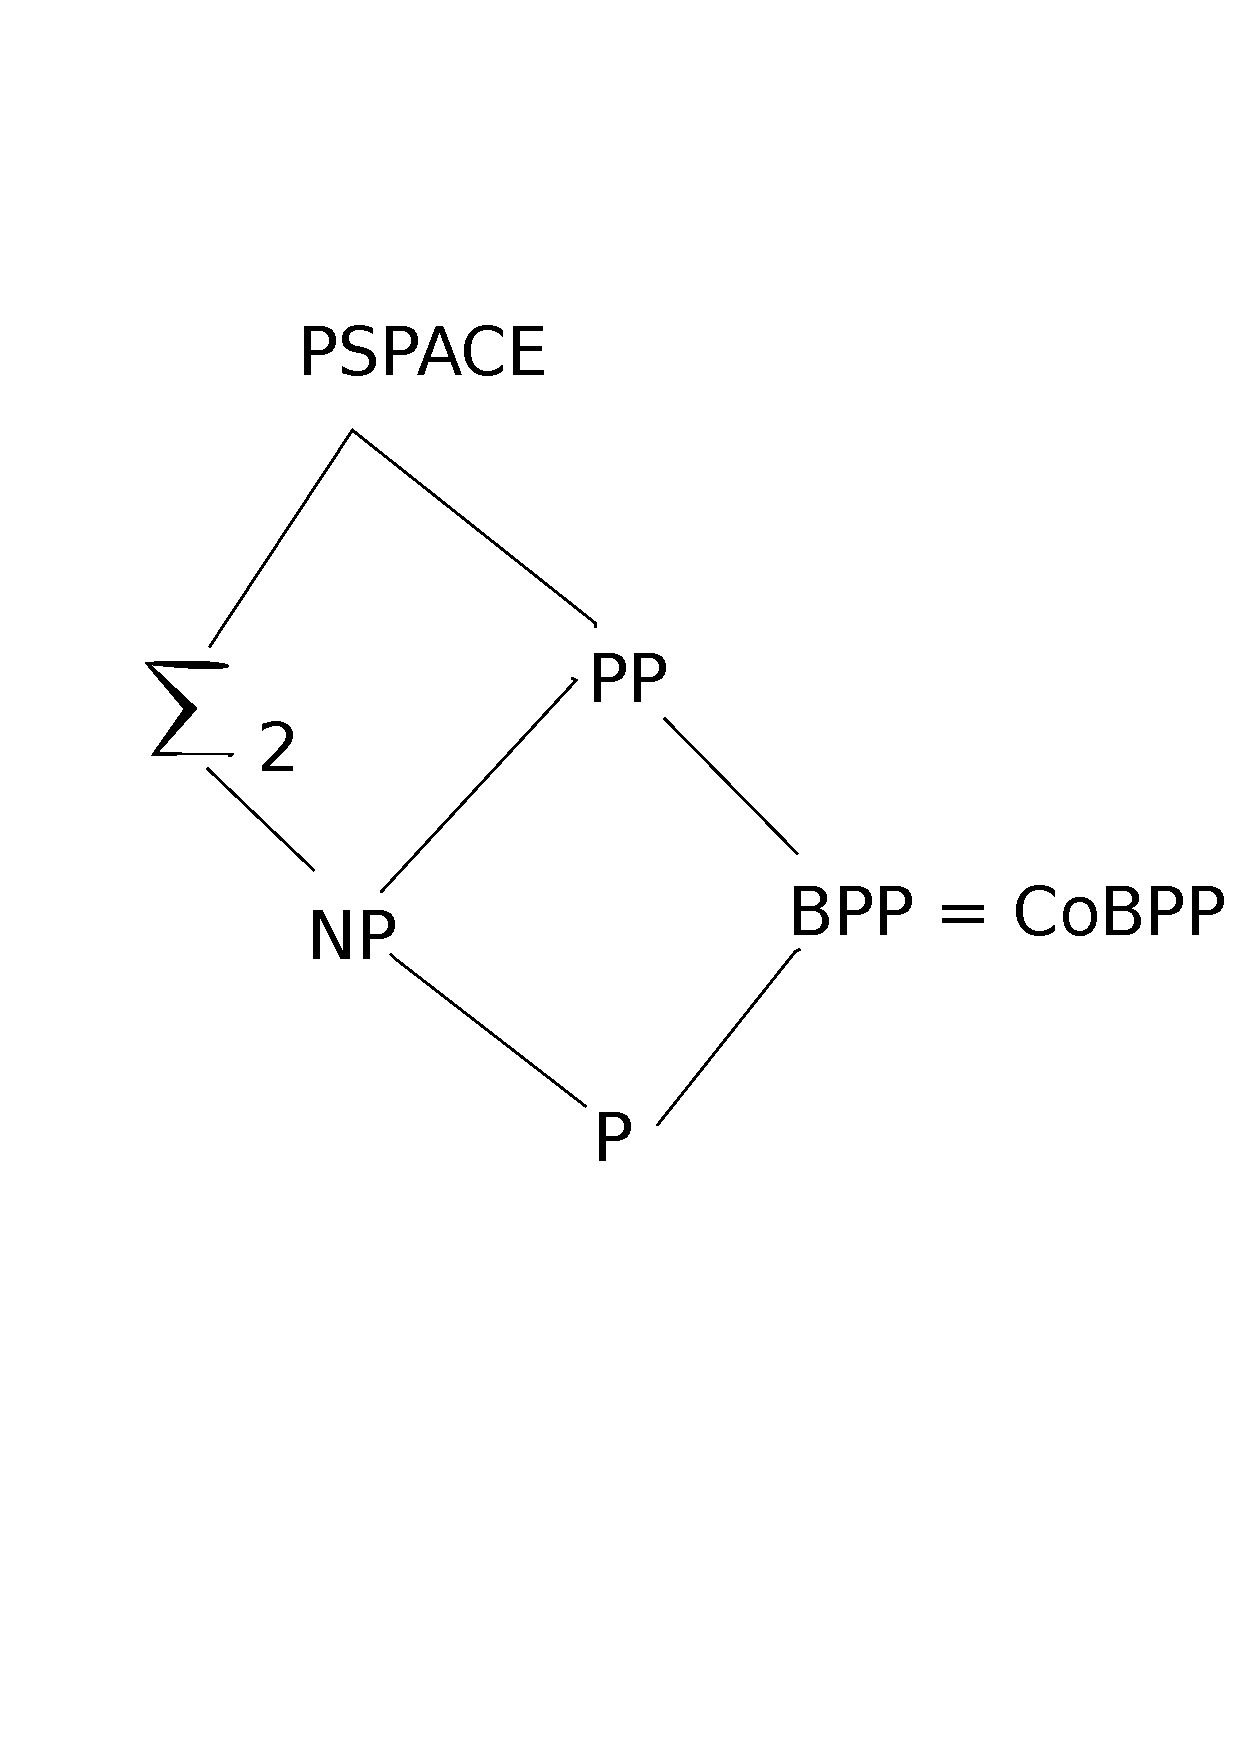
\includegraphics[scale=0.5,trim = 10mm 80mm 50mm 5mm]{hie1}
%\pagebreak

\section*{One-sided Error Randomized Algorithms}

Consider the language , PIT that is, Polynomial Identity Testing,
\[PIT =\{ p |  p\equiv 0 \}\] where $p$ is a polynomial.
From, the last lecture, we make the following observation about PIT,
if $p \in PIT$, PTM makes no error,
if $p \notin PIT$, PTM makes some error (less than half the number of paths).

We now explore how complexity theory can be extended to these kind of algorithms too.
\begin{definition}({\bf \RP})
A language $L$ is said to be in $\RP$ if there is an $\epsilon$ such
that $0 < \epsilon < \frac{1}{2}$, and a randomized algorithm $A$ such that :
\begin{eqnarray*}
x \in A & \implies & Pr [\textrm{ $A$ accepts }] \ge \frac{1}{2}+\epsilon \\
x \notin A & \implies & Pr [\textrm{ $A$ accepts }] = 0
\end{eqnarray*}
\end{definition}

Hence we have the following proposition:
\begin{equation}
PIT \in \co\RP
\end{equation}

\begin{proposition}
$\RP \subseteq \NP$
\end{proposition}
\begin{proof}
Consider language $L \in \RP$ via machine $M$ such that 
$x \in L \implies M $ accepts $x$ with some error $\epsilon < \frac{1}{2}$
$\implies M $ accepts $x$ on atleast 1 path. \\
$x \notin L \implies M$ accepts $x$ with probability 0 $\implies M$ rejects on all paths.
Thus $L \in \NP$. Moreover, even with the acceptance condition of a non-deterministic machine, the branching machine corresponding to the $\RP$ algorithm accepts the language $L$ itself.
\end{proof}
\vspace{-40mm}
\begin{center}
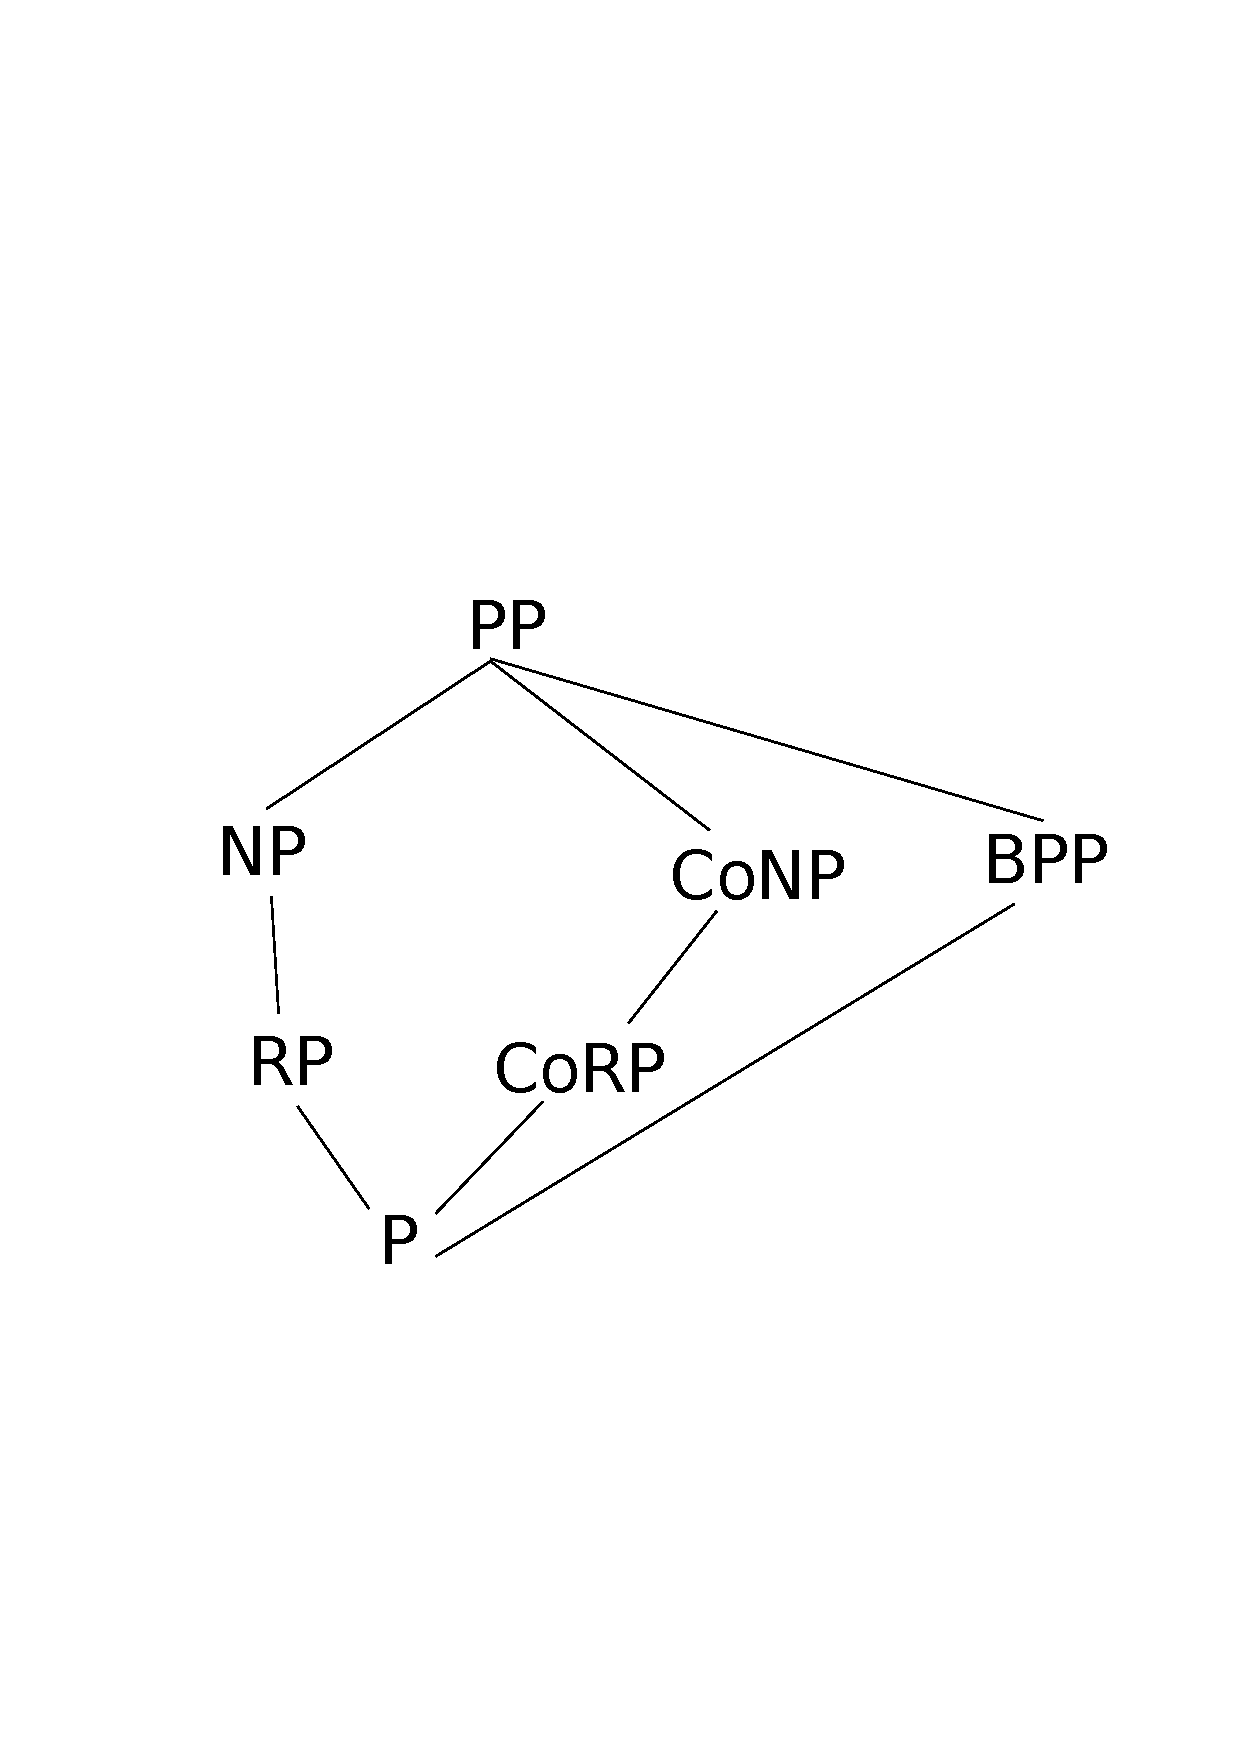
\includegraphics[scale=0.3, trim = 30mm 50mm 0mm 5mm, clip]{Lecture11-Princy/hie2}
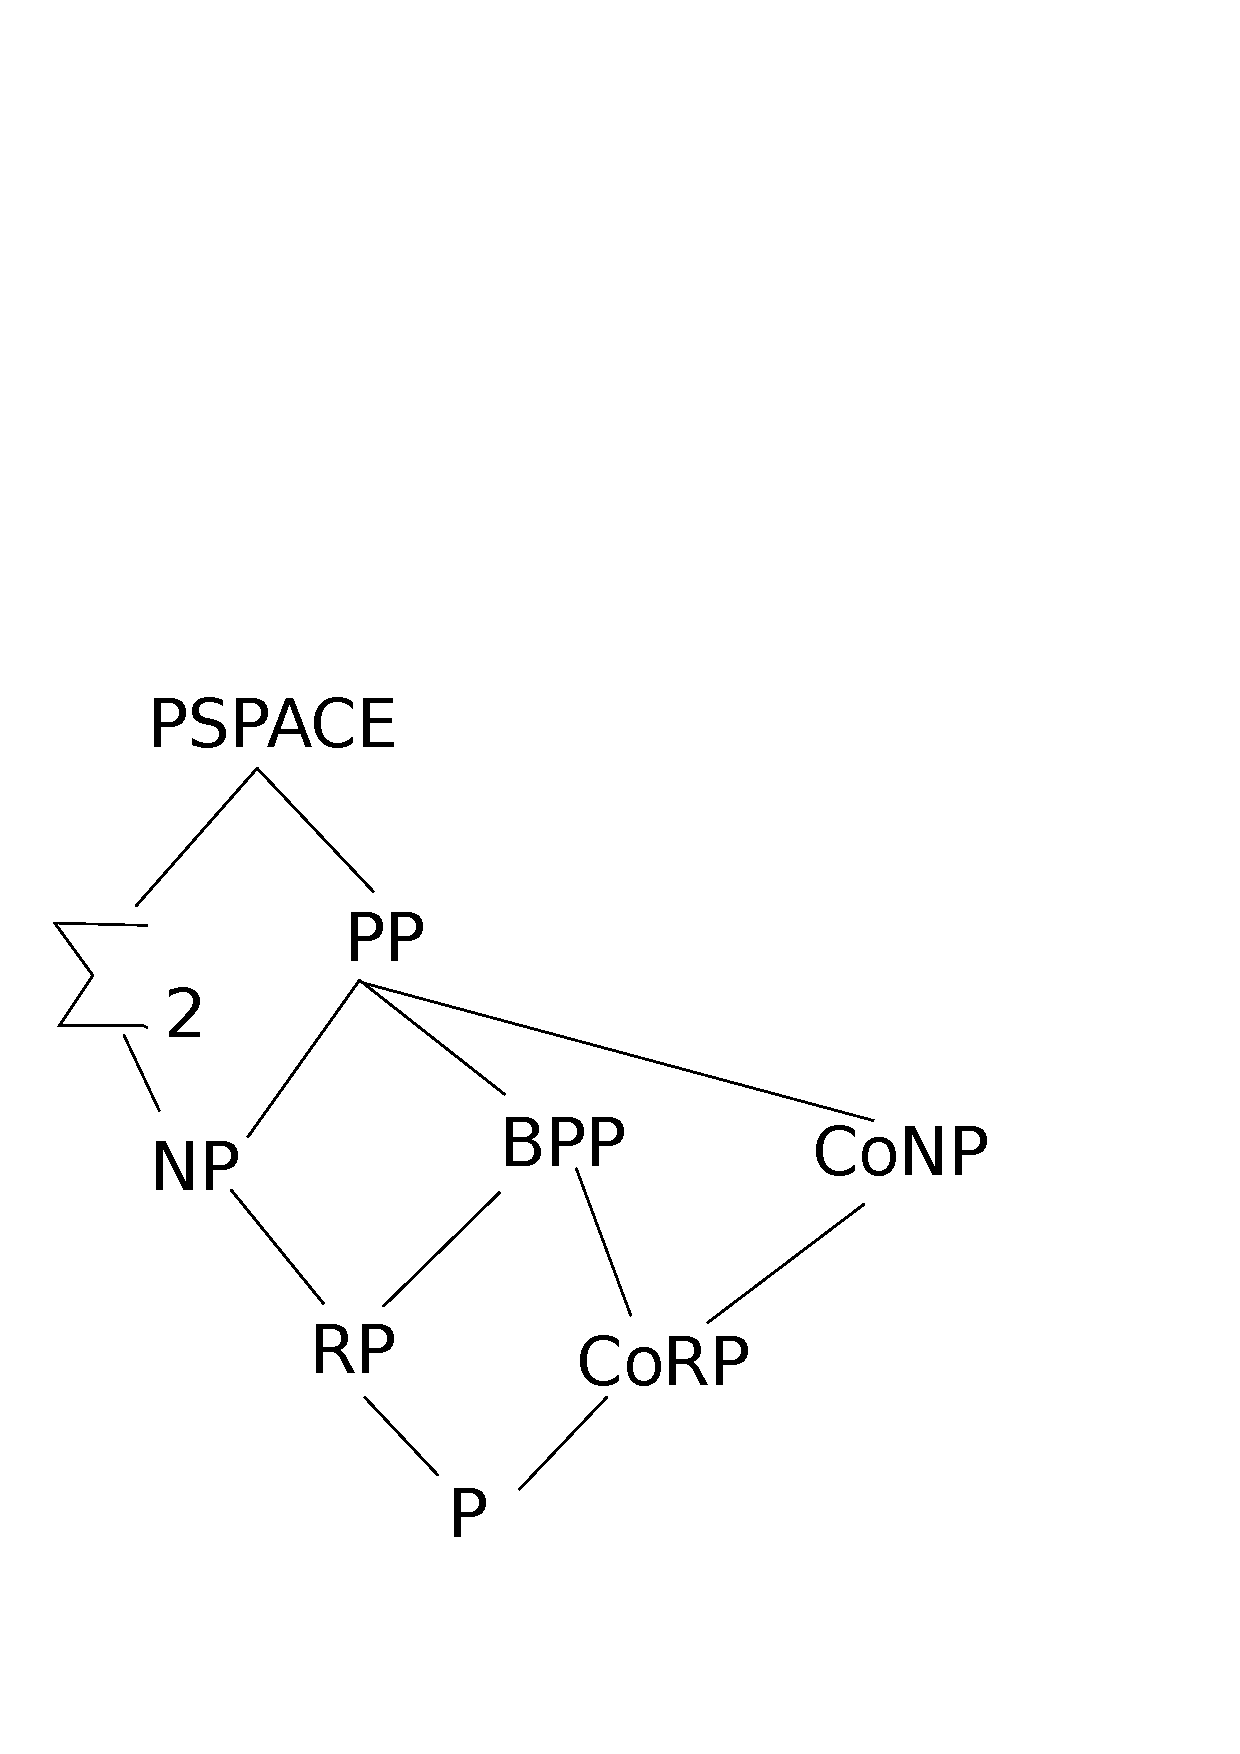
\includegraphics[scale=0.3]{Lecture11-Princy/hie3}
\end{center}
\vspace{-10mm}

\section{Derandomization of $\BPP$}
There are several questions connected to the new class $\BPP$ that contains several natural problems. We saw one example of multivariate polynomial identity testing problem. Is $BPP \subseteq P$? This would amount to showing that in the world of efficient computations, randomization does not add any power. There are reasons to remotely believe this to be the case, but till date there is no proof. 

A question of slightly different flavour is, if problems in $\BPP$ are contained in $\NP$? That is, can we trade non-determinism with randomness? We already know that if the randomness causes only one-sided error, then it can be replaced by simple non-deterministm ($\RP \subseteq \NP$). But extending this to two-sided error version is an interesting open problem in the area. 

We show a relaxed containment which can be seen to be an improved upper bound for problems in $\BPP$ compared to the trivial upper bound of $\PSPACE$.

\begin{theorem}
$BPP \in \Sigma_2$
\end{theorem}
\begin{proof}
Let $L \in \BPP$. By using amplification lemma for $q(n) = n$ we can state:
there is a probabilistic Turing machine $M$ and polynomial p(n) such that,
\[\#err_M(x) \leq 2^{-n} 2^{p(n)}\]

Let us recall the definition and a characterization of the class $\Sigma^2$
$\Sigma_2$ is defined as follows:
$L \in \Sigma_2$ iff $\exists B \in P $ such that:
\[x \in L \iff \exists y,  \forall z,  (x,y,z) \in B\]

There is a clear mindblock here. How do we tradeoff quantifiers to randomness?

Let us define a set A(x) as follows:
\[ A(x) = \{y\in \{0,1\}^{p(n)} |  M\ accepts\ x\ on\ path\ y \}\]

Observe that, 
\[x \in L \Rightarrow |A(x)| \geq (1- 2^{-n}) 2^{p(n)} \]
that is, no. of $y$'s such that $M(x,y) = 1$ is large.
\[x \notin L \Rightarrow |A(x)| \leq  2^{-n} 2^{p(n)}) \] 
that is, no, of $y$'s such that $M(x,y) = 1$ is small.
\\

\textbf{Parity Map:}
For two strings $y,z \in \{0,1\}^{p(n)}$, let $y \parity z$ denote the bit-wise parity of the two strings.
We can extend the parity map to operate on subsets of $\{0,1\}^{p(n)}$ as follows:
\[ S \parity z = \{y \parity z ~|~ y \in S \, z \in \{0,1\}^{p(n)} \}\]

\begin{observation}
For a fixed $z$, $\parity_z$ is a bijection from $\{0,1\}^{p(n)} \to \{0,1\}^{p(n)}$. That is, for any $z \in \{0,1\}^{p(n)}$, and $S \subseteq \{0,1\}^{p(n)}$, $|S| =|S \parity z|$.
\end{observation}

Ask the question : how many $z$'s do we need to cover $\{0,1\}^{p(n)}$ entirely?
That is, how large do we need $m$ to be, such that there exists strings $z_1, z_2, \ldots, z_m$ such that:
\[\bigcup_{i=1}^{m} (A(x) \parity z_i) = \{0,1\}^{p(n)}  \]

Intuitively, we expect the answer to be {\em small} when the size of $A(x)$ is large, and {\em large} when the size of $A(x)$ is small. Now we formalize this.

\textbf{Case 1:} Small $|A(x)| \leq 2^{-n} 2^{p(n)}$
In the best case, let each $z_i$ maps $A(x)$ to non-intersecting sets.
\[ \forall i, j (A(x)\parity z_i) \cap (A(x) \parity z_j) = \phi , i \neq j \]
\[|\bigcup_{i=1}^{m} (A(x) \parity z_i)| \geq |\{0,1\}^{p(n)}|\]
\[\Rightarrow m (2^{-n}) 2^{p(n)} \geq 2^{p(n)}\]
\[\Rightarrow m \geq 2^n\]

Hence, the no. of $z$'s required is exponential in $n$ when $A(x)$ is small, that is, when
$x \notin L$.
\\

\textbf{Case 2:} Large $|A(x)| \geq (1 - 2^{-n}) 2^{p(n)}$
We prove that $\exists z_1, z_2, z_3 ... z_m$ for a small $m$ such that 
\[|\bigcup_{i=1}^{m} (A(x) \parity z_i)| = |\{0,1\}^{p(n)}|\]
We call the $m$-tuple $z_1, z_2, z_3 ... z_m$ {\em bad}, if ,
\[|\bigcup_{i=1}^{m} (A(x) \parity z_i)| \neq |\{0,1\}^{p(n)}|\]
\[\Rightarrow \exists w \in \{0,1\}^{p(n)}, z_i \parity y \neq w ,\forall y \in
A(x), \forall i \]
\[\Rightarrow \{z_i \parity w | 1 \leq i \leq m \} \subset R(x)\]
where $R(x) = \bar A(x)$.
$|R(x)| = 2^{p(n)} - |A(x)|$
$\Rightarrow |R(x)| \leq  2^{p(n) - n}$

For a given $w$ and a given subset of $R(x)$ of size $m$, we get a {\em bad} $m$-tuple
$z_1, z_2, z_3 ... z_m$. Hence,
\\
Number of {\em bad} $z_1, z_2, z_3 ... z_m \leq $ Number of of $w$'s $\times$ Number of subsets
of $R(x)$ of size $m$.
\\
$\Rightarrow$ Number of {\em bad} $z_1, z_2, z_3 ... z_m \leq 2^{p(n)} (2 ^{p(n)-n})^m $
\\
Total number of $z_1, z_2, z_3 ... z_m $ = $(2^{p(n)})^m$.
$m$ should be such that,
\[2^{p(n)} (2 ^{p(n)-n})^m < (2^{p(n)})^m\]
\[p(n) + (p(n)-n)m < p(n)m\]
\[p(n) - nm < 0\]
\[m > \frac{p(n)}{n}\]

This goes well with our intuition. If $m$ is allowed to be very small, then we should not be able to cover the entire set $\{0,1\}^n$. For, $m > \frac{p(n)}{n}$ we are guaranteed to have atleast one {\em good} $m$-tuple, that is,
\[z_i \parity w = y , y \in A(x)\]

Hence we conclude that, 
\[\exists z_1, z_2, z_3 ... z_m , \forall w \in \{0,1\}^{p(n)} \left( \bigwedge_{i=1}^{m} \left[~z_i \parity w
\in A(x) ~\right] \right) \]
\[\exists z_1, z_2, z_3 ... z_m , \forall w \in \{0,1\}^{p(n)}, \left( \bigwedge_{i=1}^{m} \left[ ~M(x, z_i
\parity w) = 1 ~\right] \right) \]

Checking if $M$ accepts $x$ on a given path is a polynomial time operation, and
repeating it for each $z_i$ where the number of $z_i$'s is polynomial in $n$ is
also a polynomial time operation. Fix $m = p(n)$, Thus we have a $B \in \P$ such that

\[ x \in L \iff \exists \overline{z} \in \{0,1\}^{p(n)^2}, \forall w \in \{0,1\}^{p(n)} (x,\overline{z},w) \in B \]
Hence, the above language $L \in \Sigma_2$.
\end{proof}
  

\newpage \Lecture{Sajin Koroth}{January 28, 2012}{12}{One random string for all}
%\theme{Advice Classes and $\BPP$} 

%\lectureplan{

Today we will be
  showing an interesting consequence of amplification of $\BPP$
  introduced earlier. We will show that for an amplified $\BPP$
  algorithm there is a good string of random bits for each input
  length $n$ such that the algorithm run with these random bits is
  correct for all inputs $x$ of length $n$. Hence if you could get
  this good random string some how then you can decide a language in
  $\BPP$ in polynomial time without any randomness. But there is a
  catch, although we prove the existence of such a random string we do
  not know how to compute such a string efficiently. Hence we will
  introduce a new model of computation where you are given such advice
  strings for free, but the advice for all inputs of length $n$ has to
  be the same. We will introduce an advice string based class called
  $P/poly$, and will discuss its connection to $\BPP$
  %}

\section{One random string for all}
Recall that amplification allows to transform in polynomial time any
$\BPP$ algorithm to a $\BPP$ algorithm with error bound
$2^{-2n}$(i.e. at most $2^{-2n}$ fraction of random strings are ``bad'')
using $p(n)$ randomness. We will show that for a $\BPP$ algorithm with
the above mentioned error bound there is one random string for every
length $n$ such that for any input of that length $n$, the $\BPP$
algorithm outputs correctly on that random string. For the rest of the
lecture we will work with sufficiently amplified success probability
$\BPP$ machines, where the notion of sufficient success probability is
defined as given below :
\begin{align}
  x\in L \implies \Pr_{y} \left[ M(x,y) \text{ accepts } \right] & \geq
   1-2^{-2n} \\
  x \notin L \implies \Pr_{y}\left[ M(x,y) \text{ accepts } \right] & \geq
   2^{-2n} 
\end{align}
That is in such a machine the number of random strings $y$ which lead
the machine to output a wrong answer is bounded by $2^{-2n}$. Now let
us consider a matrix $A$ whose rows are indexed by inputs of length
$n$ and columns are indexed by random strings of length $p(n)$, and
the $(i,j)$th entry is $1$ if on fixing the random bits to be $j$ the
machine $M$ on input $i$ outputs correctly and it is $0$
otherwise. That is $A(i,j)=1$ if and only if $M(i,j)=\chi_L(i)$, where
$\chi_L(i)$ is the membership function of the language $L$
(i.e. $\chi_L(i)=1$ if and only if $i\in L$). By the amplification we
are guaranteed that for a given input $i$ at most $2^{-2n}$ fraction
of the random strings can have $A(i,j)=0$. Hence the total number of
zeros in the $A$ matrix is at most the number of rows times the
maximum number of zeros in a row, which is equal to 
\begin{eqnarray*}
  \text{\# 0's in matrix }A & \leq 2^n \times 2^{-2n} \times 2^{p(n)}
  \\
                            & \leq 2^{p(n)-n}
\end{eqnarray*}

But the total number of zeros, $2^{p(n)-n}$ is strictly less than the
number of columns in the matrix $A$. Hence there must be at least one
column with no zeros in it. If a column in the $A$ matrix has no zeros
then by the definition of $A$ matrix, the random string represented by
this column when fed as random bits to machine $M$ would output
correctly $\chi_L(x)$ for every $x\in \{0,1\}^{n}$.

\section{Class $\P/\poly$}

Even though we have proved the existence of a fixing of random bits
for an arbitrary input length $n$ of an amplified $\BPP$ machine $M$
such that the $M$ on these random bits decides all inputs $x$ of a
given length correctly for $L(M)$, we do not know how to compute such
a string efficiently (deterministically or using a randomized
algorithm) for arbitrary amplified $\BPP$ machines. Also note that the
good random string can vary with the input length. But if we can get
this random string for each input length $n$ for \textbf{free} then we
can decide a language in $\BPP$ in $\P$. That if there is a function
$h:N \to \{0,1\}^*$ such that $h(n)$ is at most polynomial in $n$ and
is the correct random string for the given $\BPP$ machine $M$, for all
inputs of length $n$, for all $n$ then we can construct a machine
$M^{'}$ such that it on input $(x,h(|x|))$ will simulate $M$ on $x$
using $h(|x|)$ as the random bits tape.

We will generalize the above ideas to define a class such that every
language in $\BPP$ is also in this class. 

\begin{definition}[$\P/\poly$]
A language $L$ is in $\P/\poly$ if there exists a polynomial $p(n)$, an
advice function $h:N\to \{0,1\}^*$ and a language $B\in \P$ such that
$\forall n,|h(n)|\leq p(n)$ and 
\begin{displaymath}
  x\in L  \iff (x,h(|x|)) \in B 
\end{displaymath}
where $|x|$ denotes the length of the string $x$.

\end{definition}

\subsection{$\BPP \subset \P/\poly$}

This is a straight forward corollary of the existence of a good random
string for any $\BPP$ machine, which works correctly for all inputs of
a given length. To show that for any $L\in \BPP$ it is also true that
$L\in \P/\poly$ we will use the fact that there a $\BPP$ machine $M_L$
accepting $L$ with error at most $2^{-2n}$ using at most $p(n)$ random
bits. We have already shown that for such a machine for every input
length $n$ at least one of $2^{p(n)}$ possible random strings is good
for all inputs of length $n$. We define the advice function $h(n)$ to
be a good random string which works for all inputs of length
$n$. Hence $|h(n)|=p(n)$ is at most polynomial in input length. Note
that definition of $P/poly$ doesn't have any requirements on the
computability of such a function, but needs the guarantee that such a
function exists. We will construct a machine $M_B$ running in
deterministic polynomial time which would accept
the language $B \in \P$ which accepts $(x,h(|x|))$ for all $x\in
L$. The machine $M_B$ on input $(x,h(|x|))$ starts simulating $M_L$ on
input $x$ using $h(|x|)$ as the random bits. By the definition of
$h(|x|)$, $M_L(x)$ using random bits $h(|x|)$ accepts if and only if
$x\in L$. Hence the proof.

\subsection{With advice comes the undecidable}

A consequence of the above definition of class $\P/\poly$ is that it not
only contains $BPP$, but it also contains some undecidable languages
as we do not insist on computability of advice function $h$. One such
undecidable language is \textbf{Unary Halting Problem} defined as 
\begin{displaymath}
  \text{UHP} = \left\{   1^n \mid \text{ Turing machine encoded by
      bin}(n) \text{ halts on all inputs}  \right\}
\end{displaymath}

It is easy to note that the general halting problem reduces to the unary
halting problem. Hence UHP is undecidable because HP is. 

We can also show that UHP is in $\P/\poly$. This is very straight
forward because the language is a unary language and there is exactly
one input of length $n$. Hence the advice function is simply a bit
representing the answer to the UHP on input $1^n$. Since we just need
a single bit of advice note that UHP is also in $\P/\theta(1)$. Also
from the above argument we can deduce that complement of UHP is also
in $\P/\poly$ because by modifying the $\P/\poly$ machine for UHP to
accept when $h(n)=0$ and reject otherwise where $h()$ is the advice
function for UHP, we get a $\P/\poly$ machine for
$\overline{\text{UHP}}$. Hence $\P/\poly$ not only contains complete
problems for semi-decidable languages, like UHP also contains
languages which are complete for co-semi-decidable languages, like
$\overline{\text{UHP}}$.



\newpage \Lecture{Sajin Koroth}{January 28, 2012}{13}{Self Reducibility of $\SAT$, Complete problem for  $\Sigma_k^\P$}
%\theme{Polynomial Hierarchy and its relation to $\P/\poly$}
%\lectureplan{
Recall that we introduced the advice based class $\P/\poly$
in the last lecture. We also saw that $\BPP \subsetneq \P/\poly$, and
by definition $\P \subsetneq \P/\poly$. But we don't know whether
$\NP\subsetneq \P/\poly$ or not. Hence if we could prove that $\NP
\not\subset \P/\poly$ then we would essentially be separating $\P$
from $\NP$. The reason why most of the complexity theorists believe $\NP
\not\subset \P/\poly$ is, if $\NP \subset \P/\poly$ then we would be
able to prove that $\PH=\Sigma_2^\P$, contrary to the common belief
that $\PH$ does not collapse. In today's lecture we will detail two
key ingredients needed for showing the above mentioned conditional
collapse of $\PH$, \textbf{a complete problem for $\Sigma_k^\P$} and
\textbf{self reducibility property of $\SAT$}
 % }

\section{Complete problem for the hierarchy}

We will first show a complete problem for the $k$th level of
polynomial hierarchy. Later on we will use the self-reducibility
nature of this problem to show the conditional collapse mentioned
earlier. Recall that a language $L$ is said to be in $\Sigma_k^\P$ 
if there exists polynomials $p_1,\dots,p_k$ and a machine $M$ running
in deterministic polynomial time such that
\begin{displaymath}
  x \in L \iff \exists y_1 \forall y_2 \exists y_3 \dots Q_k y_k
  \left[ M(x,y_1,y_2,y_3,\dots,y_k) = 1\right] , \forall i,|y_i|\leq p_i(|x|)
\end{displaymath}

Cook-Levin theorem guarantees that machine $M$ on input $x$ can be
converted into formula $\phi_x$ in polynomial time on variables
$y_1,y_2,\dots,y_k$ such that $\phi_x(y_1,y_2,y_3,\dots,y_k)$ is
satisfiable if and only if $M(x,y_1,y_2,y_3,\dots,y_k)$ accepts. Hence
we can say that the following problem is complete for $\Sigma_k^\P$,
\begin{definition}[$\Sigma_k-\SAT$] 
$\Sigma_k-\SAT$ is the set of all quantified Boolean formulas with at
most $k$ alternations (starting with an existential quantifier) which
are true. That is
\begin{displaymath}
  \Sigma_k-\SAT = \left\{ \exists y_1 \forall y_2 \exists y_3 \dots Q_k y_k
  \phi(y_1,\dots,y_k) \mid \exists y_1 \forall y_2 \exists y_3 \dots Q_k y_k
  \phi(y_1,\dots,y_k) \text{ is true} \right\}
\end{displaymath}
\end{definition}

The above problem is clearly in $\Sigma_k^\P$ as you can in polynomial
time construct from a formula, a machine in $\P$ for checking if the
formula is satisfiable or not given an assignment of all the variables
as input. The problem is $\Sigma_k^\P$ hard because
of Cook-Levin reduction from any machine in $\P$ to an equivalent formula.
 
\section{Self reducibility of $\SAT$}

Suppose we are given that $\NP \subset \P/\poly$ then we know that
there is a polynomial time deterministic Turing machine and a
polynomial length advice string for each input length such that the
machine decides a given language in $\NP$. We will sketch how this can
cause a collapse in the Polynomial Hierarchy, without giving the
details but exposing some difficulties which we have to overcome
before getting to the proof. To prove that $\PH$ collapses to
$\Sigma_2^\P$ it suffices to show that $\Sigma_3^\P=\Sigma_2^\P$. Recall
that $\Sigma_3^\P$ is the set of true quantified Boolean formulas which
are of the form $\exists y_1 \forall y_2 \exists y_3
M(x,y_1,y_2,y_3)$, and $\Sigma_2^\P$ are true quantified Boolean
formulas which are of the form $\exists y_1 \forall y_2
M(x,y_1,y_2)$. Also we are given that $\NP \subset \P/\poly$ hence for
any $L\in \NP$ there exists $h:N \to \{0,1\}^*$ and an $M\in \P$ such
that $x \in L$ if and only if $(x,h(|x|))$ is accepted by $M$. The
idea to place $\Sigma_3^\P$ in $\Sigma_2^\P$ is the following, the third
there exists $y_3$ and $M(x,y_1,y_2,y_3)$ can be combined to a machine
in $\NP$, where it first guesses a string $y_3$ of size $p_3(|y_3|)$
and then runs $M$ on $(x,y_1,y_2,y_3)$. We have assumed that
equivalent to this $\NP$ machine there is a $\P/\poly$ machine, and
even though we don't know the advice string we know there exists a
good advice string, and given the advice string the last ``there
exists'' quantifier in $\Sigma_3^\P$ can be eliminated by replacing it
with the polynomial time machine which is given the advice string,
hence we would a get a language in $\Sigma_2^\P$. But unfortunately we
don't know the advice string, hence the next best thing to do is to
guess the advice string using the first ``there exists'' quantifier in
$\Sigma_2^\P$. We are guaranteed that at least one guess is the
correct advice string. But there is a catch here, we could have
guessed the advice string incorrectly in some branch which in turn
could have led the machine $M$ to accept incorrectly thus falsely
accepting a string outside the language $L$ in $\Sigma_3^\P$. To get
around this problem we will use the first part to reduce the problem
in $\Sigma_3^\P$ to $\Sigma_3-\SAT$ and then use an algorithm for
$\SAT$ which given a sub-routine which tells a formula is satisfiable
or not, which uses a crucial property of the $\SAT$ problem,
self-reducibility to construct a satisfying assignment for the given
formula. And in the case it cannot construct a satisfying assignment
we would be able to guarantee that the advice string guessed is bad.

Self reducibility of $\SAT$ refers to the property of the $\SAT$
problem that checking a formula on $n$ variables is satisfiable
reduces to checking the satisfiability of two formulas on $n-1$
variables. This property leads to a polynomial time algorithm for
constructing a satisfying assignment given a polynomial time
sub-routine deciding the decision version of $\SAT$ problem
correctly. Algorithm~\ref{SAT_ASGN_ALGO} constructs a satisfying
assignment given a sub-routine which correctly solves $\SAT$ instances
of up to $n$ variables. Notice that one important property of
Algorithm~\ref{SAT_ASGN_ALGO} is that even if the sub-routine which
checks the satisfiability of a formula is wrong, the algorithm would
not be accepting an un-satisfiable formula as a satisfiable
formula. Because at the end of the algorithm we are checking whether
the assignment constructed by the algorithm is satisfiable or not, so
even if the sub-routine for $\SAT$, \textbf{SATISFIABLE} is
erroneous we would not be able to construct a satisfying assignment
for an un-satisfiable formula. But it might fail to construct a
satisfying assignment for a satisfiable formula if the sub-routine is
erroneous.

% Could not be added due to conflict with clrs package. Needs to be rewritten
% in algorithm 
%\begin{codebox}
%\label{SAT_ASGN_ALGO}
%  \Procname{$\proc{SATISFYING-ASSIGNMENT}(\phi(x_1,\dots,x_n))$}
%%  \li $\id{\psi(x_1,\dots,x_n)} \gets \phi(x_1,\dots,x_n)$
%  \li \For $i \gets 1$ \To $\id{n}$
%  \li \Do
%  \li $\id{\psi^{'}} \gets \psi(x_i=0)$
%  \li $\id{\psi^{''}} \gets \psi(x_i=1)$
%  \li \If $\proc(SATISFIABLE(\psi^{'}))$
%  \li \Then $\id{a_i} \gets 0$
%  \li       $\id{\psi} \gets \psi(0,x_2,\dots,x_n)$
%  \li \ElseIf $\proc(SATISFIABLE(\psi^{''}))$
%  \li \Then $\id{a_i} \gets 1$
%  \li       $\id{\psi} \gets \psi(1,x_2,\dots,x_n)$
%  \li \ElseNoIf
%  \li \Return $\const{impossible}$
%      \End
%  \li \If $\phi(a_1,\dots,a_n) = 1$ 
%  \li \Then \Return $(a_1,\dots,a_n)$
%  \li \Else \Return $\const{impossible}$
%      \End
%      \End
%\end{codebox}


\newpage \Lecture{Anup Joshi}{Jan 30, 2012}{14}{Karp-Lipton-Sipser Collapse Theorem}
%\theme{Between $\P$ and $\PSPACE$.}
%\lectureplan{ Karp-Lipton-Sipser Theorem : If $\NP$ is contained in $\P/\poly$ then $\PH$ collapses to
%$\Sigma_{2}$.}

We showed that $\BPP \subseteq \P/\poly$, and as we argued $\P/\poly$ seems to be a huge class containing $\P$ and $\BPP$, and even some undecidable languages. A natural question is whether $\NP$ is also contained in $\P/\poly$. We show that both answers to this question has interesting consequences.

Suppose we are able to prove that $\NP \not\subseteq \P/\poly$, then we are indeed are proving that $\NP \not\subseteq \P$. That is big !.

Suppose we are able to prove that $\NP \subseteq \P/\poly$. Does it have any consequences?
In this lecture, we will prove the Karp-Lipton-Sipser theorem, which says that if $\NP$ is
contained in $\P/poly$, then the polynomial hierarchy collapses to $\Sigma_{2}$. It is believed
that the polynomial hierarchy does not collapse, since the flavour of the question about each level of the hierarchy is about elimination of a quantifier, and is of a similar difficulty to to $\P$ vs $\NP$ question. 

Summarising this discussion; we believe that $\NP \not\subseteq \P$, but we do not know how to prove it. But then, since $\P \subseteq \P/\poly$ is this not a harder problem to solve that $\P vs \NP$? Yes, but why do we even bother to address it when we do not know how to attack the easier question? As we will see later in the course (when we do circuit complexity) this class $\P/\poly$ provides this nice escape from the "combinatorics of a Turing machine" and helps us to prove theorems which we do not know how to prove otherwise. It was for precisely this reason that, in the definition of $\P/\poly$ we did not make the advice function even computable (to avoid references to Turing machines).

We state the theorem.
\begin{theorem}[{\bf Karp-Lipton-Sipser, 1980}]
If $\NP \subseteq \P/\poly$, then $\PH$ collapses to $\Sigma_2$.
\end{theorem}

We prove the theorem by proving two lemmas. We first show that our assumption implies something much stronger. That is if $\NP \subseteq \P/\poly$ then not only $\NP$, but the entire $\PH$ will be in $\P/\poly$.

\begin{lemma}
 If $\NP \subseteq \P/\poly$, then $\PH \subseteq \P/\poly$.
\end{lemma}
\begin{proof}
It suffices to show that $\Sigma_{k} \subseteq \P/poly$ for any $k$. We prove this by induction on $k$.
For $k = 1$, it is trivially true, since $\Sigma_{1} = \NP$. Hence, the base case is true. Consider
an $L \in \Sigma_{2}$, then $L \in \NP^{B}$ for some $B \in \NP$. But $\NP \subseteq \P/poly$ (by
the induction hypothesis), hence, $\exists h : \mathbb{N} \rightarrow \{0, 1\}^*$ and $C \in P$,
such that, $y \in B \leftrightarrow  (y, h(y)) \in C$. Now, membership in $B$ is decidable in
polynomial time with the help of the advice function. Hence, we do not need to make oracle query to
$B$ to resolve membership questions in $L$, we can embed the polynomial time computation of the
oracle with advice function in the NTM for L itself. So we can say that, $L \in \NP$ with the advice
function $h : \mathbb{N} \rightarrow \{0, 1\}^*$. We can rewrite it as $\exists h : \mathbb{N}
\rightarrow \{0, 1\}^* \wedge C' \in \NP$ such that  $x \in L \leftrightarrow (x, h(|x|)) \in C'$.

Now, what can we say about $C'$? We know that $C' \in \NP$, hence $C' \in \P/poly$. Hence there is
an advice function for $C'$ also, so that membership in $C'$ is computable in polynomial time with
the help of that advice function. That is, $\exists g : \mathbb{N} \rightarrow \{0, 1\}^* \wedge D
\in \P$ such that  $y \in C' \leftrightarrow (y, g(|y|)) \in D$. Rewriting it we get:

\begin{center}
\begin{math}
 (x, h(|x|)) \in C' \leftrightarrow (x, h(|x|), g(p(x))) \in D
\end{math}
\end{center}

Hence from the above argument we see that $L \in \P/\poly$.
\end{proof}

Now we show that if any level of $\PH$ is in $\P\/poly$, then it essentially gives a way to express the acceptance condition using only two quantifiers. This is done in the following lemma.

\begin{lemma}
 For any $k > 2$, if $\Sigma_{k} \subseteq P/poly$, then $\Sigma_{k} \subseteq \Sigma_{2}$.
\end{lemma}
%\begin{proof-idea}
\begin{proof}
It suffices to show that $L \in \Sigma_{k} \implies L \in \Sigma_{2}$. For this, we take the
language $\SAT_{k}$ which is a quantified boolean formula with at most $k$ alternating
quantifiers. Since $\SAT_{k}$ is $\Sigma_{k}$-complete for any $k$, the lemma follows.

Let us assume that for any $k > 2$, $\Sigma_{k} \subseteq \P/\poly$. Let $L \in \Sigma_{k}$, and
since $\SAT_{k}$ is $\Sigma_{k}$-complete, then by our assumption, $\SAT_{k} \subseteq P/poly$. By
the definition of $\P/\poly$, $\exists h : \mathbb{N} \rightarrow \{0, 1\}^* \wedge B \in \P$ such that
$\phi \in \SAT_{k} \leftrightarrow (\phi, h(|\phi|)) \in B$. If $|\phi| = n$, then $h(n) \in \{0,
1\}^{p(n)}$. Let us define a new function $w$ in the following way:

\begin{center}
\begin{math}
 w = g(n) = (h(0), h(1), ..., h(n))
\end{math}
\end{center}
For any $\phi \in \Sigma_{k}$, such that $|\phi|
\leq n$, the string $w$ has the following properties:
\begin{enumerate}
\item $(0, w) \notin B$ $\wedge$ $(1, w) \in B$
\item If $\phi = \exists y, \psi \wedge \phi \in \SAT_{k}$, then $(\psi |_{y = 0}, w) \in B \vee
(\psi |_{y = 1}, w) \in B$.
\item If $\phi = \forall y, \psi \wedge \phi \in \SAT_{k}$, then $(\psi |_{y = 0}, w) \in B \wedge
(\psi |_{y = 1}, w) \in B$.
\end{enumerate}
Hence, $(\phi, w) \in B \implies 1, 2,$ and $3$ are satisfied.

It is also true in the other direction. That is, if $1, 2, $ and $3 $ are satisfied, then in order to check if $\phi$ is true, it suffices to check if $(\phi, w) \in B$. We can show this inductively. When $\phi$ is either $0$ or $1$, then by $1$, the above claim is true. Suppose, $\phi = (\exists x) \psi$, then we can apply $2$ on $\psi$ to evaluate it.
Otherwise, if $\phi = (\forall x) \psi$, then we can apply $3$ on $\psi$ to evaluate it. Thus, by recursively evaluating, we can reach upto the leaf where we apply $1$. Hence by a consistency check we can make sure that the advice does not give us a wrong answer, and indeed, if it gives a wrong answer to us, we can detect it at some point in the recursive evaluation. Note that we are using the self-reducibility property of $\SAT_k$ here.
Thus we have proved that,
\begin{center}
 \begin{math}
  \phi \in \SAT_{k} \leftrightarrow (\exists w, |w| \leq p(n)) (\forall \psi, |\psi| \leq n) (1
\wedge 2 \wedge 3 \wedge (\phi, w) \in B).
 \end{math}
\end{center}
\end{proof}


\newpage \newcommand{\USAT}{{\sf USAT}}
\Lecture{Nilkamal Adak}{Jan 31, 2012}{15}{Introduction to Toda's Theorem}
%\theme{Between $\P$ and $\PSPACE$.}
%\lectureplan{Introduce Toda's Theorem, give some relevant definitions 
%and construct a proof strategy for Toda's Theorem}

There are two different way to generalize hard problems like optimization 
problems.
\begin{enumerate}
 \item Non-determinism or quantification
 \item Counting
\end{enumerate}

It was an important open question in 1980's about relative power of those 
two approach, alternation and counting. There are various 
classes are defined independently in those two different approach. But how 
are those class comparable? In 1991, Toda came up with the following relation 
among the two different world.

\begin{theorem}
 $PH \subseteq \P^{\#\P}$
\end{theorem}
This theorem take the whole quantification world to counting world. That is 
we can solve any problem in PH in polynomial with an oracle access to 
a $\#\P$-Complete problem. Before going to the proof of Toda's theorem lets 
define the following.

\begin{definition}
$\exists.$ Operator.

Let us consider the definition of $\NP$.
\begin{center}
$L \in \NP$ if $ \exists B \in \P$ such that 
\[ x \in L \Longleftrightarrow \exists y \text{ such that } (x,y) \in B \]
\end{center}
\end{definition}
So we can think $\exists$ as an operator and let us define it as follows

Let $C$ be any class of languages. Define, 
\begin{center}
$ L \in \exists.C$  if $\exists B \in C$  such that
$x \in L \Longleftrightarrow \exists y$ such that $(x,y) \in B$
\end{center}
So $\NP = \exists .\P$

\begin{definition}
BP. Operator \\
Let us consider definition of the class $\BPP$ 

$L \in \BPP$ if $\exists B \in \P$ such that 
\begin{align*}
x \in L & \Longrightarrow {\sf Pr_y}[(x,y) \in B ] \ge \frac{3}{4} \\
x \notin L & \Longrightarrow {\sf Pr_y}[(x,y) \in B] \le \frac{1}{4}
\end{align*}
So similarly we can define BP. operator as 


\begin{center}
Let $C$ be a class of languages. 
$L \in BP.C$ if $ \exists B \in$ C such that
\begin{align*}
x \in L & \Longrightarrow {\sf Pr}[(x,y) \in B]  \ge \frac{3}{4}\\
x \notin L & \Longrightarrow {\sf Pr}[(x,y) \in B] \le \frac{1}{4}
\end{align*}
\end{center}
So $\BPP = BP.\P$
\end{definition}

Now lets define the class $\oplus \P$:
\begin{definition}
L $\in \oplus \P$ if there is a branching machine $M$ such that
\[ x \in L \Longrightarrow \#Acc_M(x) \text{ is odd} \]
\end{definition}

$\oplus\P$ can be considered as the class of decision problems corresponding 
to the least significant bit of a $\#\P$-problem. Now the natural 
question is ``Is $\NP \subseteq \oplus\P$?''.

We will see that $NP$ problems are reduced to $\oplus\P$ in some extend.
Lets now define Randomize Reduction as follows
\begin{definition}
$A \le B$ via a randomize reduction function $\sigma$ if 
\begin{enumerate}
\item  $\sigma$ is computable by choosing a random string 
$y \in \{0,1\}^{p(n)}$.
\item $x \in L \iff \sigma_y(x) \in B$ with high probability.
\end{enumerate}
\end{definition}

We will see that $\NP$ problems are reduced to some $\oplus\P$ problem 
via randomize reduction. More specifically $\NP \subseteq BP.(\oplus \P)$.
Now we will develop the proof strategy for Toda's theorem. 
We will proof the theorem in the following steps $\ldots$ 
\[
\NP \subseteq BP.(\oplus \P) \subseteq \BPP^{\oplus \P} \subseteq 
\P^{\#\P}=\P^{\PP} \]
Then by induction on the number of quantifiers we will show that the 
entire $PH \subseteq \P^{\#\P}$.

So our first step is to show $\NP \subseteq BP.(\oplus \P)$.

To prove this claim let us define the following languages \ldots.
\begin{definition} 
\[ \oplus \SAT = \{ \phi : \# \text{ of satisfying assignment of }
\phi \text{ is odd} \}\]
\end{definition}

Let us define the following promise problem \USAT as,
\begin{definition}
For all boolean formulas $\phi$,
\begin{align*}
\phi & \in \USAT \Longrightarrow \#SAT(\phi)=1\\
\phi & \notin \USAT \Longrightarrow \#SAT(\phi)=0
\end{align*}
\end{definition}

This is a promise problem as we will consider only those $\phi$ which 
falls into above two cases. Now we introduce a very important result called 
\emph{Valiant-Vazirani lemma} proved by Valiant and Vazirani in 1986.

\begin{lemma}(Valiant-Vazirani Lemma) \\
There exists a randomize reduction $\sigma_y$ such that
\begin{align*}
\phi & \in \SAT \iff Pr_y[\sigma_y(\phi) \in \USAT] \ge \frac{3}{4}\\
\phi & \notin \SAT \iff Pr_y[\sigma_y(\phi) \in \USAT] \le \frac{1}{4}
\end{align*}
\end{lemma}
We will prove this lemma in the next lecture and using this lemma 
we will prove our first step $\NP \subseteq BP.(\oplus\P)$.

\newpage \documentclass[11pt]{article}
\input{preamble.tex}

\begin{document}
\lecture{16}{Valiant-Vazirani Lemma}{Feb 2, 2012}{Jayalal Sarma}{Rahul CS}
\theme{NP $\subseteq$ BP.($\oplus$P)}
%\lectureplan{Randomized Reduction from SAT to $\oplus$SAT}

%SAT $\leq^{m}_{r}$ $\oplus$ SAT

In the last lecture, we outlined an approach to prove Toda's theorem. One of the key ingredients was a partial answer to the question that we had in one of the earlier lectures. Is $\NP$ contained in $\oplus\P$? In the last lecture we viewed $\exists$, $\oplus$, $\BP$ as operators on complexity classes and stated that $\NP$ is contained in $\BP.(\oplus\P)$. 
We also interpreted this in the following way; there is a randomized reduction from $\SAT$ to a language in $\oplus\P$.

\section{Randomized Reduction from SAT to $\oplus$SAT}
Define languages, 
\begin{itemize}
\item[]USAT=$\{\phi \mid \#\phi=1\}$ \newline where $\#\phi$ is the number of satisfying assignments to the formula $\phi$
\item[]$\oplus$SAT=$\{\phi \mid \exists k \in \mathbb{N}, \#\phi=2k+1\}$
\end{itemize}

The following Lemma, famously known as the Valiant-Vazirani Lemma, was proved by Valiant and Vazirani in 1986. It proved instrumental for many results later, including Toda's theorem which we will be taking up in the next lecture.

The lemma states the following reduction from $\SAT$ to $USAT$. 

\begin{lemma}[{\bf Valiant-Vazirani Lemma}]
There exists a randomized polynomial time algorithm that takes input $\phi$ and produces a formula $\psi_{\phi,y}$ (say $\psi$) such that,
\begin{eqnarray*}
\phi \in \SAT \implies Pr(\psi \in USAT) & \geq & \frac{1}{8n} \\
\phi \not\in \SAT \implies Pr (\psi' \not\in USAT) & = & 1
\end{eqnarray*}
\end{lemma}

Clearly, $\psi \in$ USAT $\Rightarrow \psi \in \oplus$ SAT. In the other case since $\psi \notin \SAT$, it is also case that $\psi \notin \oplus\SAT$. Thus as a corollary to the lemma, we get:

\begin{corollary}
There exists a randomized polynomial time algorithm that takes input $\phi$ and produces a formula $\psi$ such that,
\begin{eqnarray*}
\phi \in \SAT \implies Pr(\psi \in \oplus\SAT) & \geq &  \frac{1}{8n} \\
\phi \not\in \SAT \implies Pr (\psi \not\in \oplus\SAT) & = & 1
\end{eqnarray*}
\end{corollary}

\begin{proof}
We present a high-level idea first. Given $\phi$, a natural approach to produce a formula with unique satisfying assignment is to add another conjunction to produce $\psi = \phi \land (\omega)$ such that $\omega$ 
filters out the satisfying assignments using the clause $\omega$ such that only one of them will satisfy the resulting formula. Clearly, if $\phi$ is not satisfiable, then by construction, $\psi$ is also not satisfiable, no matter what $\omega$ is. Consider the case when $\phi$ is satisfiable. Thus, we want $\omega$ to state a property which only one of the satisfying assignments have. 

We use hashing to achieve this. That is, we will make $\omega$ state that $h(x) = 0^k$ where $0^k$ is in range of the hash family and $x$ is an assignment. The probability that there is a collision at $0^k$ for two $x$s that satisfy $\phi$ (that is, probability that two assignments that satisfy $\phi$ also satisfies $\omega$) can be controlled by choosing a nice hash family. Thus our filter, with high probability, filters out a unique satisfying assignment for $\psi$ from the set of satisfying assignments of $\phi$.

Usually, we design hash families with a size parameter $k$; the size up to which we want to guarantee collision-free property. But here we do not know the size of the subset (the set of satisfying assignments) a priori for which we are trying to achieve unique mapping(collision-free). The smaller the subset the smaller the range (of the hash functions) that we can work with. Let us say we choose randomly the number $k$ such that the number of satisfying assignments is between $2^k$ and $2^{k+1}$ and then decide hash function for all subsets of that size. Since the number of satisfying assignments could be any number from $0$ to $2^n$, we have already lost out a bit on the probability but by a factor of at most $\frac{1}{n}$.

Now we will formally address this intuition.
Let $T \subseteq \{0,1\}^n$ be the set of satisfying assignments of $\phi$. Select $k \in \{0,1,...,n-1\}$ such that $2^k \leq |T| \leq 2^{k+1}$. Let $H_{n,k}$ be a collection of functions $h: \{0,1\}^n \mapsto \{0,1\}^k$. $H_{n,k}$ is said to be pairwise independent if for every $x$,$x' \in \{0,1\}^n$ with $x \neq x'$ and for every $y$,$y' \in \{0, 1\}^k$, 
\[ \underset{h \in_R H_{n,k}}{Pr}[h(x) = y \wedge h(x') =y'] = \frac{1}{2^k}.\frac{1}{2^k}=2^{ -2k}
\]
Construct a family of pairwise independent hash functions $H_{n,k+2}$. Hence, 
\[
\stackrel{Pr}{_{h \in H,x \in T}}[h(x)=0^{k+2}]=\frac{1}{2^{k+2}}
\]

We calculate the probability of existence of a hash function $h \in H$ such that $h$ maps exactly one satisfying assignment $x \in T$ to 0$^{k+2}$. This parameter is given by,
\[
\stackrel{Pr}{_{h \in H}}[|\{x \mid x \in T, h(x)=0^{k+2}\}|=1]
\]

Once we have an $h$ satisfying the above condition, the number of satisfying assignments for $\phi$ will be exactly 1. That is, in the described transformation, if $\omega$ is $h(x)=0^{k+2}$, the number of satisfying assignments for $\psi$ will be exactly 1, if it is satisfiable. Note that we can consider the computation sequence of the hash function $h$ on a turing machine and convert that to a SAT formula using Cook-Levin reduction. We claim that,  
\[
\stackrel{Pr}{_{_{_{h \in H}}}}[|\{x \mid x \in T, h(x)=0^{k+2}\}|=1] \geq \frac{1}{8}
\]
Consider, 
\begin{eqnarray*}
\stackrel{Pr}{_{_{_{h \in H}}}}[\exists x \in T, h(x)=0^{k+2} \wedge \underset{x' \in T,x' \neq x}\forall h(x') \neq 
0^{k+2}] & & \\
\end{eqnarray*}

\begin{eqnarray*}
= & \stackrel{Pr}{_{_{_{h}}}}[\underset{x' \in T,x' \neq x}\forall h(x') \neq 0^{k+2} \mid h(x)=0^{k+2}].\stackrel{Pr}{_{_{_{h}}}}[h(x)=0^{k+2}] & \\
= & (1-\stackrel{Pr}{_{_{_{h}}}}[\underset{x' \in T,x' \neq x}\exists h(x') = 0^{k+2}|h(x)=0^{k+2}]).\stackrel{Pr}{_{_{_{h}}}}[h(x)=0^{k+2}] & \\
= & (1-\stackrel{\sum}{_{_{_{_{\stackrel{x' \in T}{x' \neq x}}}}}}\stackrel{Pr}{_{_{_{h}}}}[h(x')=0^{k+2}\mid h(x)=0^{k+2}]).\stackrel{Pr}{_{_{_{h}}}}[h(x)=0^{k+2}] & \\
\end{eqnarray*}

Let us calculate the first part of the expression, $(1-\stackrel{\sum}{_{_{_{_{\stackrel{x' \in T}{x' \neq x}}}}}}\stackrel{Pr}{_{_{_{h}}}}[h(x')=0^{k+2} \mid h(x)=0^{k+2}])$. Since $h$ is sampled from a family of pairwise independent hash functions, $h$ satisfies the condition of simple uniform hashing. That is, the events $h(x)=0^{k+2}$ and $h(x')=0^{k+2}$ are independent. Therefore,
\[
\stackrel{\sum}{_{_{_{_{\stackrel{x' \in T}{x' \neq x}}}}}}\stackrel{Pr}{_{_{_{h}}}}[h(x')=0^{k+2} \mid h(x)=0^{k+2}])=\stackrel{\sum}{_{_{_{_{\stackrel{x' \in T}{x' \neq x}}}}}}\frac{1}{2^{k+2}}= |T-\{x\}|.\frac{1}{2^{k+2}}
\]
We bound the expression from above by bounding $|T-\{x\}|$ from above. That is,
\[
\stackrel{\sum}{_{_{_{_{\stackrel{x' \in T}{x' \neq x}}}}}}\stackrel{Pr}{_{_{_{h}}}}[h(x')=0^{k+2}\mid h(x)=0^{k+2}]) \leq (2^{k+1}-1) \frac{1}{2^{k+2}}
\]
Hence, 
\begin{eqnarray*}
(1-\stackrel{\sum}{_{_{_{_{\stackrel{x' \in T}{x' \neq x}}}}}}\stackrel{Pr}{_{_{_{h}}}}[h(x')=0^{k+2}\mid h(x)=0^{k+2}]) 
& \geq & 1-(2^{k+1}-1)\frac{1}{2^{k+2}} \\
& = & 1-\frac{1}{2}[\frac{(2^{k+1}-1)}{2^{k+2}}] \\
& \geq & \frac{1}{2}
\end{eqnarray*}
Therefore, 
\[
(1-\stackrel{\sum}{_{_{_{_{\stackrel{x' \in T}{x' \neq x}}}}}}\stackrel{Pr}{_{_{_{h}}}}[h(x')=0^{k+2}|h(x)=0^{k+2}]).\stackrel{Pr}{_{_{_{h}}}}[h(x)=0^{k+2}]\geq \frac{1}{2}\cdot \frac{1}{2^{k+2}}
\]

Thus, 
\[
|T|.(1-\stackrel{\sum}{_{_{_{_{\stackrel{x' \in T}{x' \neq x}}}}}}\stackrel{Pr}{_{_{_{h}}}}[h(x')=0^{k+2}\mid h(x)=0^{k+2}]).\stackrel{Pr}{_{_{_{h}}}}[h(x)=0^{k+2}] \geq  |T|.\frac{1}{2}\frac{1}{2^{k+2}} 
\]
By bounding $|T|$ from below, the probability that there is a $x \in T$ which uniquely gets mapped to $0^{k+2}$ is given by,
\[
|T|.(1-\stackrel{\sum}{_{_{_{_{\stackrel{x' \in T}{x' \neq x}}}}}}\stackrel{Pr}{_{_{_{h}}}}[h(x')=0^{k+2}\mid h(x)=0^{k+2}]).\stackrel{Pr}{_{_{_{h}}}}[h(x)=0^{k+2}]\geq\frac{1}{2^{k}}\frac{1}{2}\frac{1}{2^{k+2}} \geq \frac{1}{8}
\]

Considering the fact that $k \in \{0,1,...,n-1\}$ satisfies $2^k \leq |T| \leq 2^{k+1}$ with probability $\frac{1}{n}$ we get,
\[
\phi \in \SAT \implies \stackrel{Pr}{_{_{_{x}}}}[\psi_{\phi,x} \in USAT] \geq \frac{1}{8n}
\]
\[
\phi \not\in \SAT \implies \stackrel{Pr}{_{_{_{x}}}}[\psi_{\phi,x} \not\in USAT] = 1
\]
\end{proof}

Now we make comments about amplification of success probability. Since the algorithm is one-sided error, an approach will be to simply repeat the experiment some $\ell$ times, and take the $\lor$ of the results. This however, causes loss of uniqueness of the assignment since different $h$ may make different $x$s to go to $0^k$. However, we can still preserve the parity with high probability that results in the following amplification result which we state as a Lemma.

\begin{lemma}
There exists a randomized polynomial time algorithm that takes input $\phi$ and produces a formula $\psi'$ such that,
\begin{eqnarray*}
\phi \in \SAT \implies Pr(\psi' \in \oplus\SAT) & \geq & 1-\frac{1}{2^{q(n)}} \\
\phi \not\in \SAT \implies Pr (\psi' \not\in \oplus\SAT] & = & 1
\end{eqnarray*}
\end{lemma}

The OR amplification says, that we report that $\phi \in \oplus\SAT$ if and only if at least one of the trials produces a formula in $\oplus\SAT$. But then, can we produce a single formula $\psi'$ such that if $\phi$ is in $\SAT$, then $\psi'$ is in $\oplus\SAT$ with high probability. We will address such a reduction in the next lecture.


Note that it is an open problem to boost the probability of $\frac{1}{8n}$ in the Valiant-Vazirani reduction to USAT.%\textbf{Attempt to Amplify:}
\end{document}

\newpage \Lecture{Princy Lunawat, Karthik Abhinav}{Feb 6, 2012}{17}{Reductions to $\oplus$-\SAT : Amplified version}
%\theme{}
%\lectureplan{}

The last few lectures focus on the Toda's theorem which states
that $\PH \subseteq \P^{\#\P}$. The first half of the proof of the theorem
shows a randomized reduction from $\PH$ to $\parity \SAT$. 

We proved the Valiant-Vazirani lemma which stated a randomized polynomial time algorithm that takes in a formula $\phi$ and produces a new formula $\psi$ such that it gives a {\em weak form} of a randomized reduction from $\SAT$ to $U\SAT$.  We have the following 
\begin{eqnarray*}
\phi \in \SAT & \implies & Pr \left( \psi \in \textrm{\sc U\SAT} \right) \ge \frac{1}{8n} \\
\phi \notin \SAT & \implies & Pr \left( \psi \notin {\sc U\SAT} \right) = 1
\end{eqnarray*}

We also concluded that this gives a weak\footnote{The reduction is weak because the error probability($1-\frac{1}{8n}$) is much more than what is allowed in a randomized reduction ($\frac{1}{2}$)} randomized reduction from $\NP$ to $\parity\SAT$.  Now we show how to amplify the success probability in the case of the reduction to $\parity \SAT$. \footnote{Such an amplification is not known for the case of $U\SAT$.}

Indeed, something special about $\parity$ is going to help us. In this lecture, we explore some properties of the $\parity$ quantifier which are used to come up with a formula $\phi''$ from a given formula $\phi \in \SAT $ such that $\phi'' \in \parity \SAT$ with high probability. We thereby deduce that $\NP <^m_r \parity \SAT$.

\section{Parity Addition, Complementation and Multiplication}
Given two boolean formulae, $\phi $ and $\phi'$, their parity can be added as follows: 
\[\parity(\phi + \phi')(\bar z) = \parity(z_0 = 0 \wedge \phi) \vee \parity(z_1 = 0 \wedge \phi')  \]
Similarly, the parity can be complemented as: 
\[(z= 0 )\wedge (\sim x_1 \wedge \sim x_2 \wedge \ldots \wedge \sim x_n ) \vee (\phi \wedge z = 1)\]
which is represented as $\phi + 1$.
Multiplication of parity is obtained as: 
\[\parity \phi(\bar z) \times \parity \phi'(\bar z) = \parity (\phi(\bar z) \wedge \phi'(\bar z)) \]
\section{Randomized Reduction}

	In our construction for the Valiant-Vazirani Lemma , we defined a formula $\psi_i = \phi \wedge (h_i(x)= 0^k)$
where $x$ is an assignment of $\phi$.Now consider a formula $\phi' = \overset{l-1}{\underset{i = 0} \wedge } (\parity
\psi_i)$. if Pr$\left[\psi_i \in \texttt{USAT} \right] \geq \frac{1}{8n}$, then Pr$\left[ \phi' \in \SAT\right] = 1 -
\left(1 - \frac{1}{8n } \right)^l]$. We now come up with a formula $\phi''$ equivalent to $\phi'$ such that the parity
of $\phi''$  is odd. that is, $\phi'' \in \parity \SAT$ conditioned on the probability that atleast one $\psi_i \in
\parity \SAT $.\\
For simplicity, consider $\psi_1$ and $\psi_2$, one of which is in $\parity \SAT$.We observe that both ,
$\psi_1 + 1$ and $\psi_2 + 1$ cannot have an odd parity. Therefore,we have, 
\begin{align*}
\parity(\psi_1 + 1) .(\psi_2 + 1) =& 0\\
\parity((\psi_1 + 1) .(\psi_2 + 1)+ 1) =& 1 
\end{align*}
Hence, $((\psi_1 + 1) .(\psi_2 + 1)+ 1) \in \parity \SAT$.In general , 
$\overset{l-1}{ \underset{i = 0}\wedge} ((\psi_i + 1)+ 1) \in \parity \SAT$ which is our new formula $\phi''$
equivalent to $\phi.$ Hence , Pr$\left[\phi'' \in \parity \SAT \right]$ is the same as that of atleast one $\psi_i$
having an odd parity.
 \[\phi \in \SAT \Rightarrow Pr \left[\phi'' \in \parity \SAT \right] =1 -\left(1 - \frac{1}{8n }\right)^l \]

To amplify this probabilty to $1 - 2^{-m} $ we choose an appropriate value of $l$ such that,
\[1 -\left(1 - \frac{1}{8n }\right)^l \geq 1 - 2^{-m} \]

Hence, we have 
\begin{eqnarray*}
 \phi \in \SAT & \Rightarrow &  Pr\left[\phi'' \in \parity \SAT \right]\geq  1 - 2^{-m} \\
 \phi \notin \SAT & \Rightarrow & Pr\left[\phi'' \in \parity \SAT \right] = 0 
\end{eqnarray*}

Hence, $\NP <^m_r \parity \SAT$.
 


\newpage \documentclass[11pt]{article}
\usepackage{amsmath,amssymb,amsfonts,amsthm,complexity}
\usepackage{verbatim}
\newcommand{\CYCLE}{{\sf CYCLE~}}
\newcommand{\FPSPACE}{{\sf FPSPACE~}}
\usepackage{tikz}
\usetikzlibrary{calc,through,backgrounds,decorations.pathmorphing}

\input{./preamble.tex}
\begin{document}
\lecture{18}{Proof of Toda's Theorem}{Feb 07, 2012}{ Jayalal Sarma
M.N.}{Sunil K.S., Kartik Abhinav}  \theme{Between P and PSPACE}
\lectureplan{In this lecture we will be concluding the lectures on the
  theme of contrasting the power of counting to that of
  alternations. Today we will be proving the interesting result that
  $\PH \subseteq \P^{\#\P}$. To do this, first using the
  Valiant-Vazirani lemma we will show that $\PH \subseteq
  \BP(\parity\P)$.}
\section{Valiant-Vazirani Lemma}
We have already saw Valiant-Vazirani theorem which stated that :
\begin{lemma} Valiant-Vazirani Theorem: There exists a probabilistic
polynomial-time algorithm f such that for every n-variable boolean
formula $\varphi$
\begin{eqnarray*}
  \varphi\in SAT\Rightarrow Pr[f(\chi)\in \parity SAT] &\geq& \frac{1}{8n} \\
  \varphi\notin SAT\Rightarrow Pr[f(\chi)\in \parity SAT] &=& 0
\end{eqnarray*}
\end{lemma}
But to prove that $\PH \subseteq \BP(\parity\P)$ we will need
amplified version of this lemma.
\begin{lemma}
Valiant-Vazirani lemma (Amplified version): There exists a randomized
algorithm which produce $\varphi$ from a given boolean formula $\phi$
such that for a polynomial $q(n)$:
\begin{eqnarray*}
  x\in L \Rightarrow Pr[\varphi\in \parity SAT] &\geq&
  \left(1-\frac{1}{2^{q(n)}}\right) \\ 
  x\notin L \Rightarrow Pr[\varphi\in \parity SAT] &\leq& \left(\frac{1}{2^{q(n)}}\right)
\end{eqnarray*}
\end{lemma}

\section{Toda's Theorem: $\PH\subseteq\P^{\#\P}$} Any problem in $\PH$
can be solved by a $\P$ machine by making queries to a $\#\P$ oracle.\newline

\textbf{Proof} \newline
This theorem will be proved in two parts
\begin{itemize}
 \item 
 $\PH\subseteq\BP(\parity\P)$
 \item
 $\BP(\parity\P) \subseteq \P^{\#P}$
\end{itemize}

% This part has been untouched. Should be modified
\textbf{Claim}: $\PH\subseteq\BP(\parity\P)$
\begin{proof} Proof by induction on the number of alterations, $k$.\\
  Basis: for $k=0$, we already have the result
  $\NP\subseteq\BP(\parity\P)$.\\ Assume the result for $k$. ie;
  $\Sigma_k$ or $SAT_k$ $\in \BP(\parity\P)$.\\ We need to prove that
  $SAT_{k+1}\in \BP(\parity\P)$.

  Consider a language L $\in \Sigma_{k+1}^{p}$, 
  $$ x \in L \Leftrightarrow \exists y_{1} \forall y_{2} (y_{1},y_{2}) \in B$$ where $B \in \Sigma_{k}^{p}$
  
  From inductive hypothesis, there exists a formula $\phi(x)$ such that $B$ can be reduced to $\parity \SAT$. \\
  Consider the formula ,
  $$\phi_{1}(x,y_{1},y_{2}) = \phi(x) \wedge (h_{1}(y_{2}) = 0^{k_{2}}) \wedge (h_{2}(y_{1}) = 0^{k_{1}})$$
  where $h_{i}(x)$ is chosen from a pairwise independent hash family. \newline
  
  Now, using the techniques seen in last lecture, reduce this formula $\phi_{1}(x,y_{1},y_{2})$ to a formula $\psi(x)$ in $\parity \SAT$. \newline
  Hence, 
    $$ x \in L \Leftrightarrow \psi(x) \in \parity \SAT$$
    Therefore, from induction, $\PH \leq_{r} \parity \P$.\newline
    $\PH \subseteq \BP(\parity \P)$
  
 \begin{comment} 
 $$\phi\in SAT_k\Rightarrow Pr[\parity_z\phi\land\tau(x,z)]\geq(1-\frac{1}{2^{q(n)}})$$
$$\phi\notin SAT_k\Rightarrow Pr[\parity_z\phi\land\tau(x,z)]\leq \frac{1}{2^{q(n)}}   $$
Now, any $\phi '\in SAT_{k+1}$ can be written as $\phi
'=\exists\sigma$ where $\sigma\in SAT_k$
$$\phi '\in SAT_{k+1}\Rightarrow\exists\sigma\in SAT_k\mbox{ with } \sigma\in\Pi_k$$

Let $\sigma '=\exists(\lnot\varphi)$ where $\sigma=\lnot\varphi$\\
$$\lnot(\forall\varphi)\Rightarrow\exists\sigma\Rightarrow Pr[\sigma '\in\parity SAT]\geq (1-\frac{1}{2^{q(n)}})$$
$$\forall\varphi\Rightarrow\lnot\exists\sigma\Rightarrow Pr[\sigma '\notin\parity SAT]\geq (1-\frac{1}{2^{q(n)}})$$
From inductive hypothesis,
$$\forall\varphi\Rightarrow Pr[\sigma ''\in\parity SAT]\geq (1-\frac{1}{2^{q(n)}})$$
$$\lnot\forall\varphi\Rightarrow Pr[\sigma ''\notin\parity SAT]\geq (1-\frac{1}{2^{q(n)}})$$
$$\varphi\rightarrow\varphi\land(h(y)=0^k)\rightarrow\varphi\land(h(y)=0^{k_1}\land h(x)=0^{k_2})$$
$$\phi=\exists\forall\varphi$$
\end{comment}

\end{proof}

%End of untouched part

\textbf{Claim}: $\BP(\parity\P) \subseteq \P^{\#\P}$

Before proving the above claim, let us set up a following lemma. \newline

Let $A \in \parity \P$, then by definition, \newline
$$x \in A \implies \#acc_{M}(x) = -1~(mod~2)$$ 
$$x \notin A \implies \#acc_{M}(x) = 0~(mod~2)$$

But what Toda argued was that, not only does this hold true under modulo 2 operation, but under any modulo $2^{q(n)}$ operation where q(n) is a polynomial.

\begin{lemma}
 Let $A \in \parity \P$, then , \newline
$$x \in A \implies \#acc_{M}(x) = -1~(mod~2^{q(n)})$$ 
$$x \notin A \implies \#acc_{M}(x) = 0~(mod~2^{q(n)})$$
 
\end{lemma}
\begin{proof}
 Let y = $\#acc_{M}(x)$,where M is the NDTM corresponding to the $\parity \P$ function f, such that f(x) = y. \newline
 $$x \in A \implies y = -1~(mod~2^{q(n)})$$ 
$$x \notin A \implies y = 0~(mod~2^{q(n)})$$
 
 Now construct a polynomial m = $3y^{4}~+~4y^{3}$. Using the NDTM M(where $\#acc_{M}(x) = m$), construct a new NDTM M' such that,
 $$\#acc_{M'}(x) = m$$
 
  To construct such a NDTM, let us look at the following two constructions
  \begin{itemize}
   \item 
    Construction of a machine M such that , $\#acc_{M}(x) = \#acc_{M_{1}}(x) + \#acc_{M_{2}}(x)$ \newline
    Describe the NDTM M as its choice tree as follows : \newline
    1) Create a new root node such that the machine can take two choices on it. \newline
    2) On one of the choices, simulate the machine $M_{1}$.\newline
    3) On the other choice, simulate machine $M_{2}$. \newline
    4) Extend the leaves of the corresponding choice tree to balance the height. \newline
    
    This new choice tree will have $\#acc_{M}(x) = \#acc_{M_{1}}(x) + \#acc_{M_{2}}(x)$.
    \item
    Construction of a machine M such that , $\#acc_{M}(x) = \#acc_{M_{1}}(x) \times \#acc_{M_{2}}(x)$ \newline
    Describe the NDTM M as its choice tree as follows : \newline
    1) Create a choice tree of either machine $M_{1}$ or $M_{2}$. W.L.G., lets assume the choice tree of machine $M_{1}$. \newline
    2) On each of the accept node of machine $M_{1}$, extend the tree downwards by simulating the machine $M_{2}$.\newline
    3) On the reject nodes, extend the tree downwards to balance the height of the choice tree. \newline
    
    This new choice tree will have $\#acc_{M}(x) = \#acc_{M_{1}}(x) \times \#acc_{M_{2}}(x)$.
    
  \end{itemize}
  
  Using the above two constructions, a NDTM M' can be constructed from machine M. \newline \newline
  Observe that, \newline
   $$x \in A \implies y = -1~(mod~2^{2})$$ 
   $$x \notin A \implies y = 0~(mod~2^{2})$$ 
    via the NDTM M'
    
  Repeating the above procedure at the  $i^{th}$ iterations, we will have,
    $$x \in A \implies y = -1~(mod~2^{2^{i}})$$ 
    $$x \notin A \implies y = 0~(mod~2^{2^{i}})$$ 
    
  Hence, repeating the procedure for O($\log(q(n)$) iterations, we will have ,
    $$x \in A \implies y = -1~(mod~2^{q(n)})$$ 
    $$x \notin A \implies y = 0~(mod~2^{q(n)})$$ 
  
  
  \textbf{Note}: \newline
  An important observation in the proof is that, the height of the choice tree increases by a factor of 4 in every iteration. Hence, the height
  of the choice tree in the final machine is $4^{\log(q(n))}$ , which is a polynomial. Hence, the running time of the finally obtained choice machine
  is also polynomial and hence the function corresponding to it, still remains in $\parity \P$.
\end{proof}

Now, using the above lemma, lets prove $\BP(\parity\P) \subseteq \P^{\#\P}$ which will complete the proof of Toda's Theorem. \newline

Consider $L \in \BP(\parity\P)$ \newline
By definition,
$$ Pr_{y\in \{0,1\}^{p(n)}} (x \in L \Leftrightarrow (x,y) \in A) \geq \frac{3}{4}$$ for some A $\in \parity \P$ \newline

Consider h(x) = $|\{y:(x,y) \in A\}|$ \newline

If we calculate the value of h(x) and estimate it to be greater than a fraction of $\frac{3}{4}$ , then accept x, else reject.\newline
Hence, L $\in \P^{\#\P}$. \newline

To estimate this value consider the function,
$$ l(x) = \Sigma_{y\in \{0,1\}^{p(n)}} acc_{M}(x,y)$$
This can be written as,
$$ l(x) = \Sigma_{(x,y) \in A} acc_{M}(x,y) + \Sigma_{(x,y) \notin A} acc_{M}(x,y)$$
$$ l(x) = (-1) \times h(x) + 0 (mod 2^{q(n)})$$
$$ l(x) = -h(x) (mod 2^{q(n)})$$

If we choose a large enough value of $2^{q(n)}$ , then we can determine value of h(x) uniquely from l(x). Formally, 
 h(x) $< 2^{q(n)}$ \newline
 
 We can easily see that function l(x) $\in \#\P$. i.e. Create an NDTM $M'$ , which first guesses nondeterministically a string $y \in \{0,1\}^{p(n)}$,
 and simulates $M$ on $(x,y)$. The number of accepting paths of the machine $M'$ is precisely equal to l(x).


\begin{comment}
\begin{lemma}
\label{lemma1} If $\mathcal{A}\in \parity\P$ then $\exists B$ such
that for any polynomial $q$ and input $x$ of length $n$,
$$x\in \mathcal{A}\Rightarrow (\#(x,y)\in B)\equiv -1 \mod 2^{q(n)}$$
$$x\notin \mathcal{A}\Rightarrow (\#(x,y)\in B)\equiv 0 \mod 2^{q(n)}$$

Now we can state the lemma as, Let $\mathcal{A}\in \parity\P$. Then
for any polynomial $q$, there exists a polynomial-time NTM M such that
for any input $x$ of length $n$,
$$x\in \mathcal{A}\Rightarrow (\chi_M(x))\equiv -1\mod 2^{q(n)}$$
$$x\notin \mathcal{A}\Rightarrow (\chi_M(x))\equiv 0 \mod 2^{q(n)}$$
Here $\chi_M(x)$ denotes the number of accepting computations of $M$
on $x$.
\end{lemma}
\begin{proof} Let $M_1$ be a polynomial time NTM such that
$$\chi_{M_1}\equiv 1\mod 2\mbox{ if } x\in \mathcal{A}$$ %and
$$\chi_{M_1}\equiv 0\mod 2 \mbox{ if }x\notin \mathcal{A}$$ 

In other words,
$$x\in \mathcal{A}\Rightarrow (\#acc_M(x)) \mbox{ is odd}$$
$$x\notin \mathcal{A}\Rightarrow (\#acc_M(x))\mbox{ is even}$$


Define another polynomial time NTM $M_2$ that repeats $M_1$ on $x$ a
number of times such that
$$x\in \mathcal{A}\Rightarrow (\#acc_{M_2}(x)) \mbox{ is odd}$$
$$x\notin \mathcal{A}\Rightarrow (\#acc_{M_2}(x))\mbox{ is even}$$

Note: Given two NDTMs $M_1$ and $M_2$, we know how to get an $M_3$
with:
\begin{itemize}
\item $\#acc_{M_3}(x)=\#acc_{M_1}(x)+\#acc_{M_2}(x) $: By running
$M_1$ and $M_2$ in parallel.
\item $\#acc_{M_3}(x)=\#acc_{M_1}(x)\times\#acc_{M_2}(x) $: By rnning
$M_1$ and $M_2$ one after other.
\end{itemize}

Let $f(x,i)=\chi_{M_2}(<x,i>)$. It if clear that $f$ satisfies the
recurrence relation given below:
\begin{eqnarray}
\label{rec} f(x,i+1)=3f(x,i)^4+4f(x,i)^3, i\geq0
\end{eqnarray} From equation ~\ref{rec}
$$f(x,0)\mbox{ is even }\Rightarrow f(x,i)\equiv 0\mod 2^{2^i}$$
$$f(x,0)\mbox{ is odd }\Rightarrow f(x,i)\equiv -1\mod 2^{2^i}$$
Now from the above analysis,
$$x\in \mathcal{A}\Rightarrow (\chi_M(x)\equiv  -1\mod 2^{2^{\log q(n)}}\equiv -1\mod 2^{q(n)}$$
$$x\notin \mathcal{A}\Rightarrow (\chi_M(x)\equiv  0\mod 2^{2^{\log q(n)}}\equiv 0\mod 2^{q(n)}$$
\end{proof}


\begin{theorem} $\BP(\parity\P)\subseteq \P^{\#\P}$
\end{theorem}
\begin{proof} $L\in \BP(\parity\P)$ means there exists a set
$\mathcal{A} \in \parity\P$ and a polynomial $p$ such that for all
$x$,
$$x\in L \Rightarrow Pr_y[(x,y)\in \mathcal{A}]\geq \frac{2}{3}$$
$$x\notin L \Rightarrow Pr_y[(x,y)\in \mathcal{A}]\leq \frac{1}{3}$$
where $y$ ranges over all strings of length $p(|x|)$.

By lemma ~\ref{lemma1}, if $\mathcal{A} \in \parity\P$, there exists a
polynomial-time NTM M such that for all $(x,y)$, with $|x|=n$ and
$|y|=p(n)$
$$\chi_M(<x,y>)\equiv -1\mod 2^{p(n)}, \mbox{ if } <x,y>\in\mathcal{A}$$
$$\chi_M(<x,y>)\equiv 0\mod 2^{p(n)}, \mbox{ if } <x,y>\notin\mathcal{A}$$


Let $g(x)$ and $h(x)$ are two functions defined as,
\begin{eqnarray*} g(x)=|\{y:|y|=p(|x|),(x,y)\in \mathcal{A}\}|\\
h(x)=\displaystyle\sum_{|y|=p(|x|)}\chi_M(<x,y>)
\end{eqnarray*} Then for any $x$ of length $n$,
\begin{eqnarray*}
h(x)&=&\displaystyle\sum_{<x,y>\in\mathcal{A}}\chi_M(<x,y>)+\displaystyle\sum_{(<x,y>\notin\mathcal{A})}\chi_M(<x,y>)\\
&=&(\displaystyle\sum_{<x,y>\in\mathcal{A}}(-1)+\displaystyle\sum_{(<x,y>\notin\mathcal{A})}0)\mod
2^{q(n)}\\ %&\equiv&(g(x).(-1)+(2^{p(n)}-g(x)).0)\mod 2^{p(n)}\\
&\equiv&(g(x).(-1)+(2^{p(n)}-g(x)).0)\mod 2^{p(n)}\\
&\equiv&(-g(x))\mod 2^{p(n)}
\end{eqnarray*} Construct a machine $N$ that has $h(x)$ accepting path
(Just guess a $y$ and run $N$). Now make a query to a $\#\P$ machine
to compute $h(x)$. By having $q(n)$ sufficiently large, ie.,
$2^{q(n)}>2{p(n)}$ we can compute $g(x)=(2^{p(n)}-h(x))$.

We know $x\in L$ if and only if $g(x)>2^{p(n)-1}$. Since $g(x)$ can be
computed from $h(x)$ and $p(n)$ it is clear that we can decide whether
$x\in L$ from $h(x)$. The function $h$ is in $\#\P$, we can define an
NTM $M_1$ that on input $x$ first nondeterministically guesses a
string $y$ of length $p(|x|)$ and then simulate $M$ on $<x,y>$.
Hence, $L\in P^{\#\P}$.
\end{proof}

\end{comment}

\end{document}



\bibliographystyle{abbrv}
\bibliography{references}

\end{document}
